\subsection{\label{sec:calib.ec}Electrocalorimeter Calibration and Resolution}
The timing calibration of the EC system was performed using the ecGammaCal package, using photon hits. This package has been used by multiple running groups, although not all groups. An example of the method, shown in Fig.~\ref{ectall}, compares the photon vertex time according to EC, and the event vertex time. This calibration process uses real photon hits to perform the calibration on a iterative basis by improving the definition of good photon hits using prior calibration constants. Once the preliminary results are obtained, the stability of the calibration constants are monitored on a run-by-run, basis. The integrated results are  shown in Fig.~\ref{ectrunsec} for sector 1 as an example. Clearly, the whole running period can be devided into several stable running periods to obtain the final calibration constants. The quality of the calibration for these individual ranges can be seen in Fig.~\ref{ectrun}. The timing resolution in Fig.~\ref{ectrun} are shown to be about $700$~ps, instead of $500$~ps, due to the fact that in the inclusion of background hits in the EC that are not photons.

\begin{figure}[h]
\begin{center}
 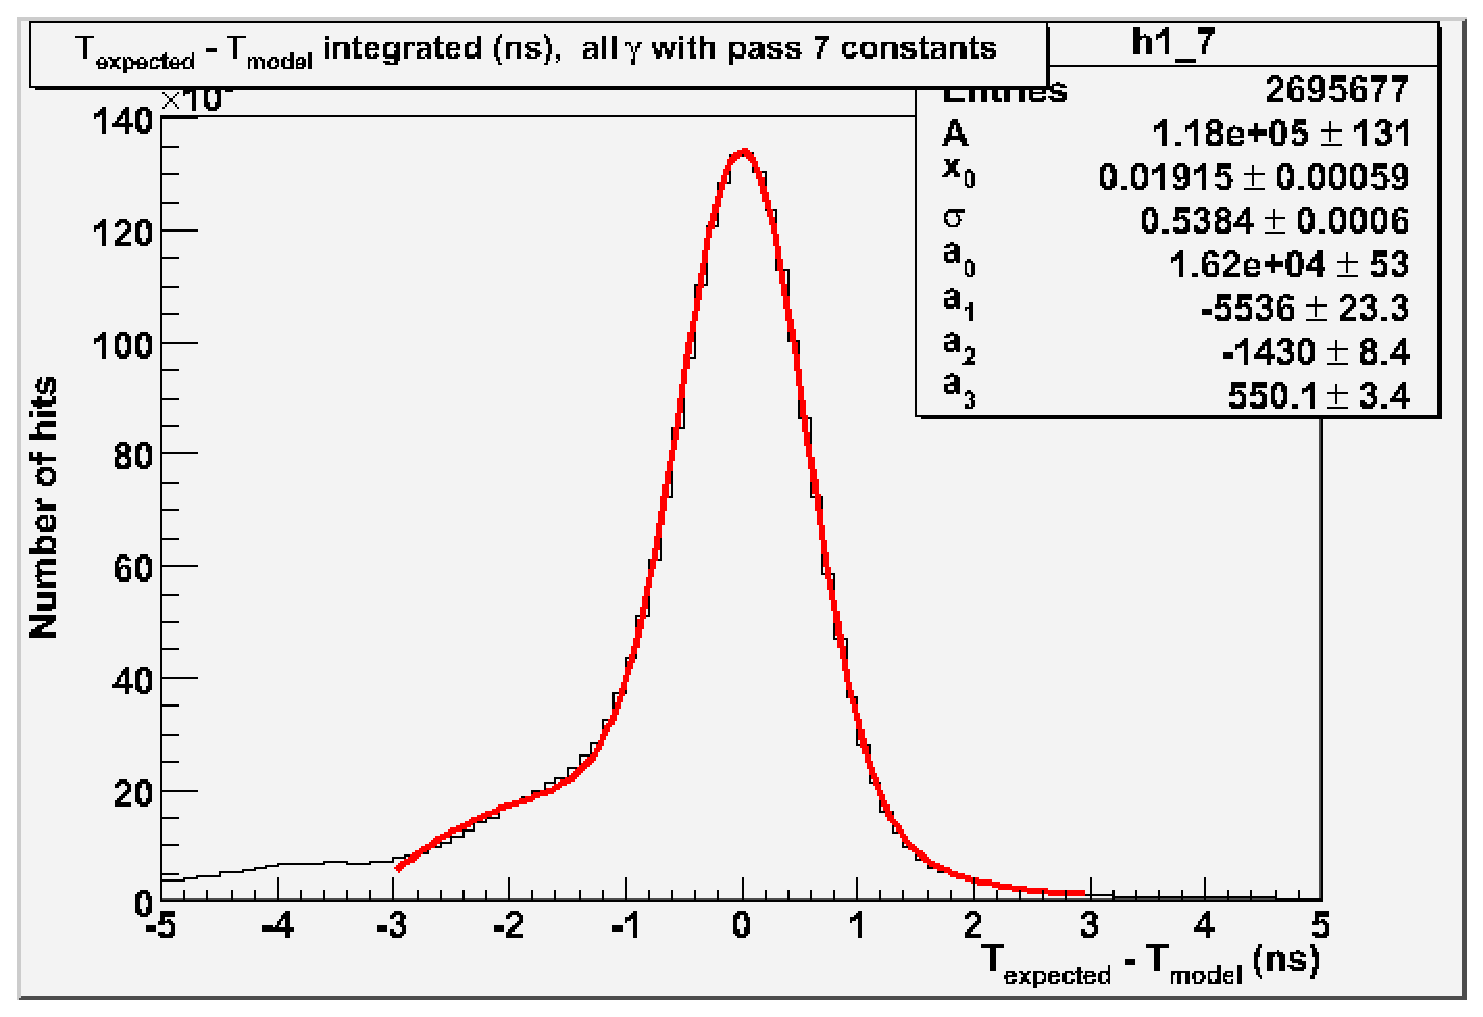
\includegraphics[width=0.45\textwidth]{figures/calib/ec/ec_vtimeall.eps}
  \caption{And example of the EC calibration plot, comparing  the difference between photon vertex time according to EC ($T_{model}$, and according to the event vertex time($T_{expected}$), to obtain the EC timing calibration constants. The resolution, integrated for all tubes, are about $500$~ps, for good photon candidates}
  \label{ectall}
  \end{center}
\end{figure}


\begin{figure}[h]
\begin{center}
 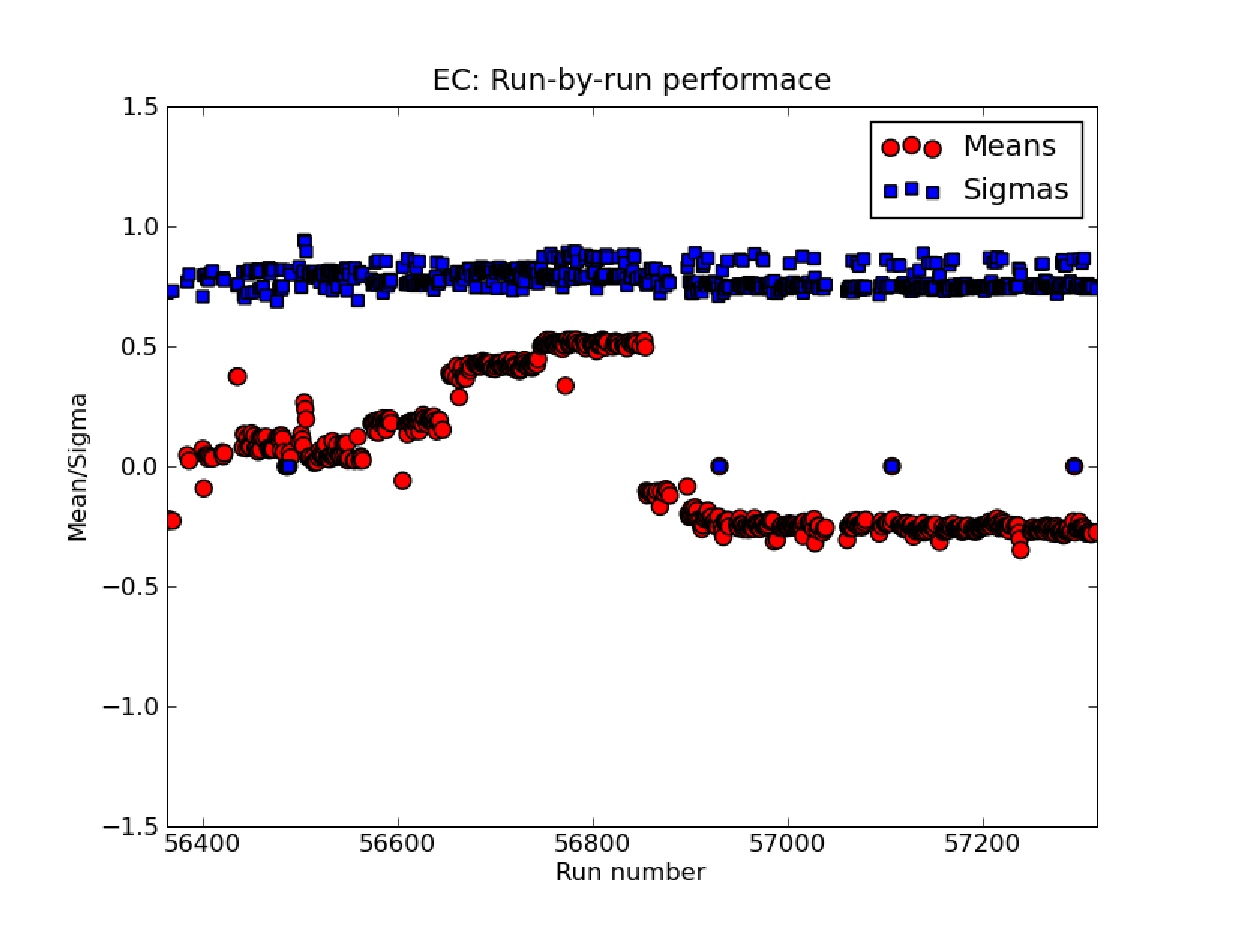
\includegraphics[width=0.45\textwidth]{figures/calib/ec/ec_vtimebyrunsec.eps}
  \caption{An example of the ec timing calibration before the final results, i.e., the mean and $\sigma$ of the photon vertex time according to EC, and the event vertex time, as a function of the run numbers. Only sector 1 is shown here.}
  \label{ectrunsec}
  \end{center}
\end{figure}

\begin{figure}[h]
\begin{center}
 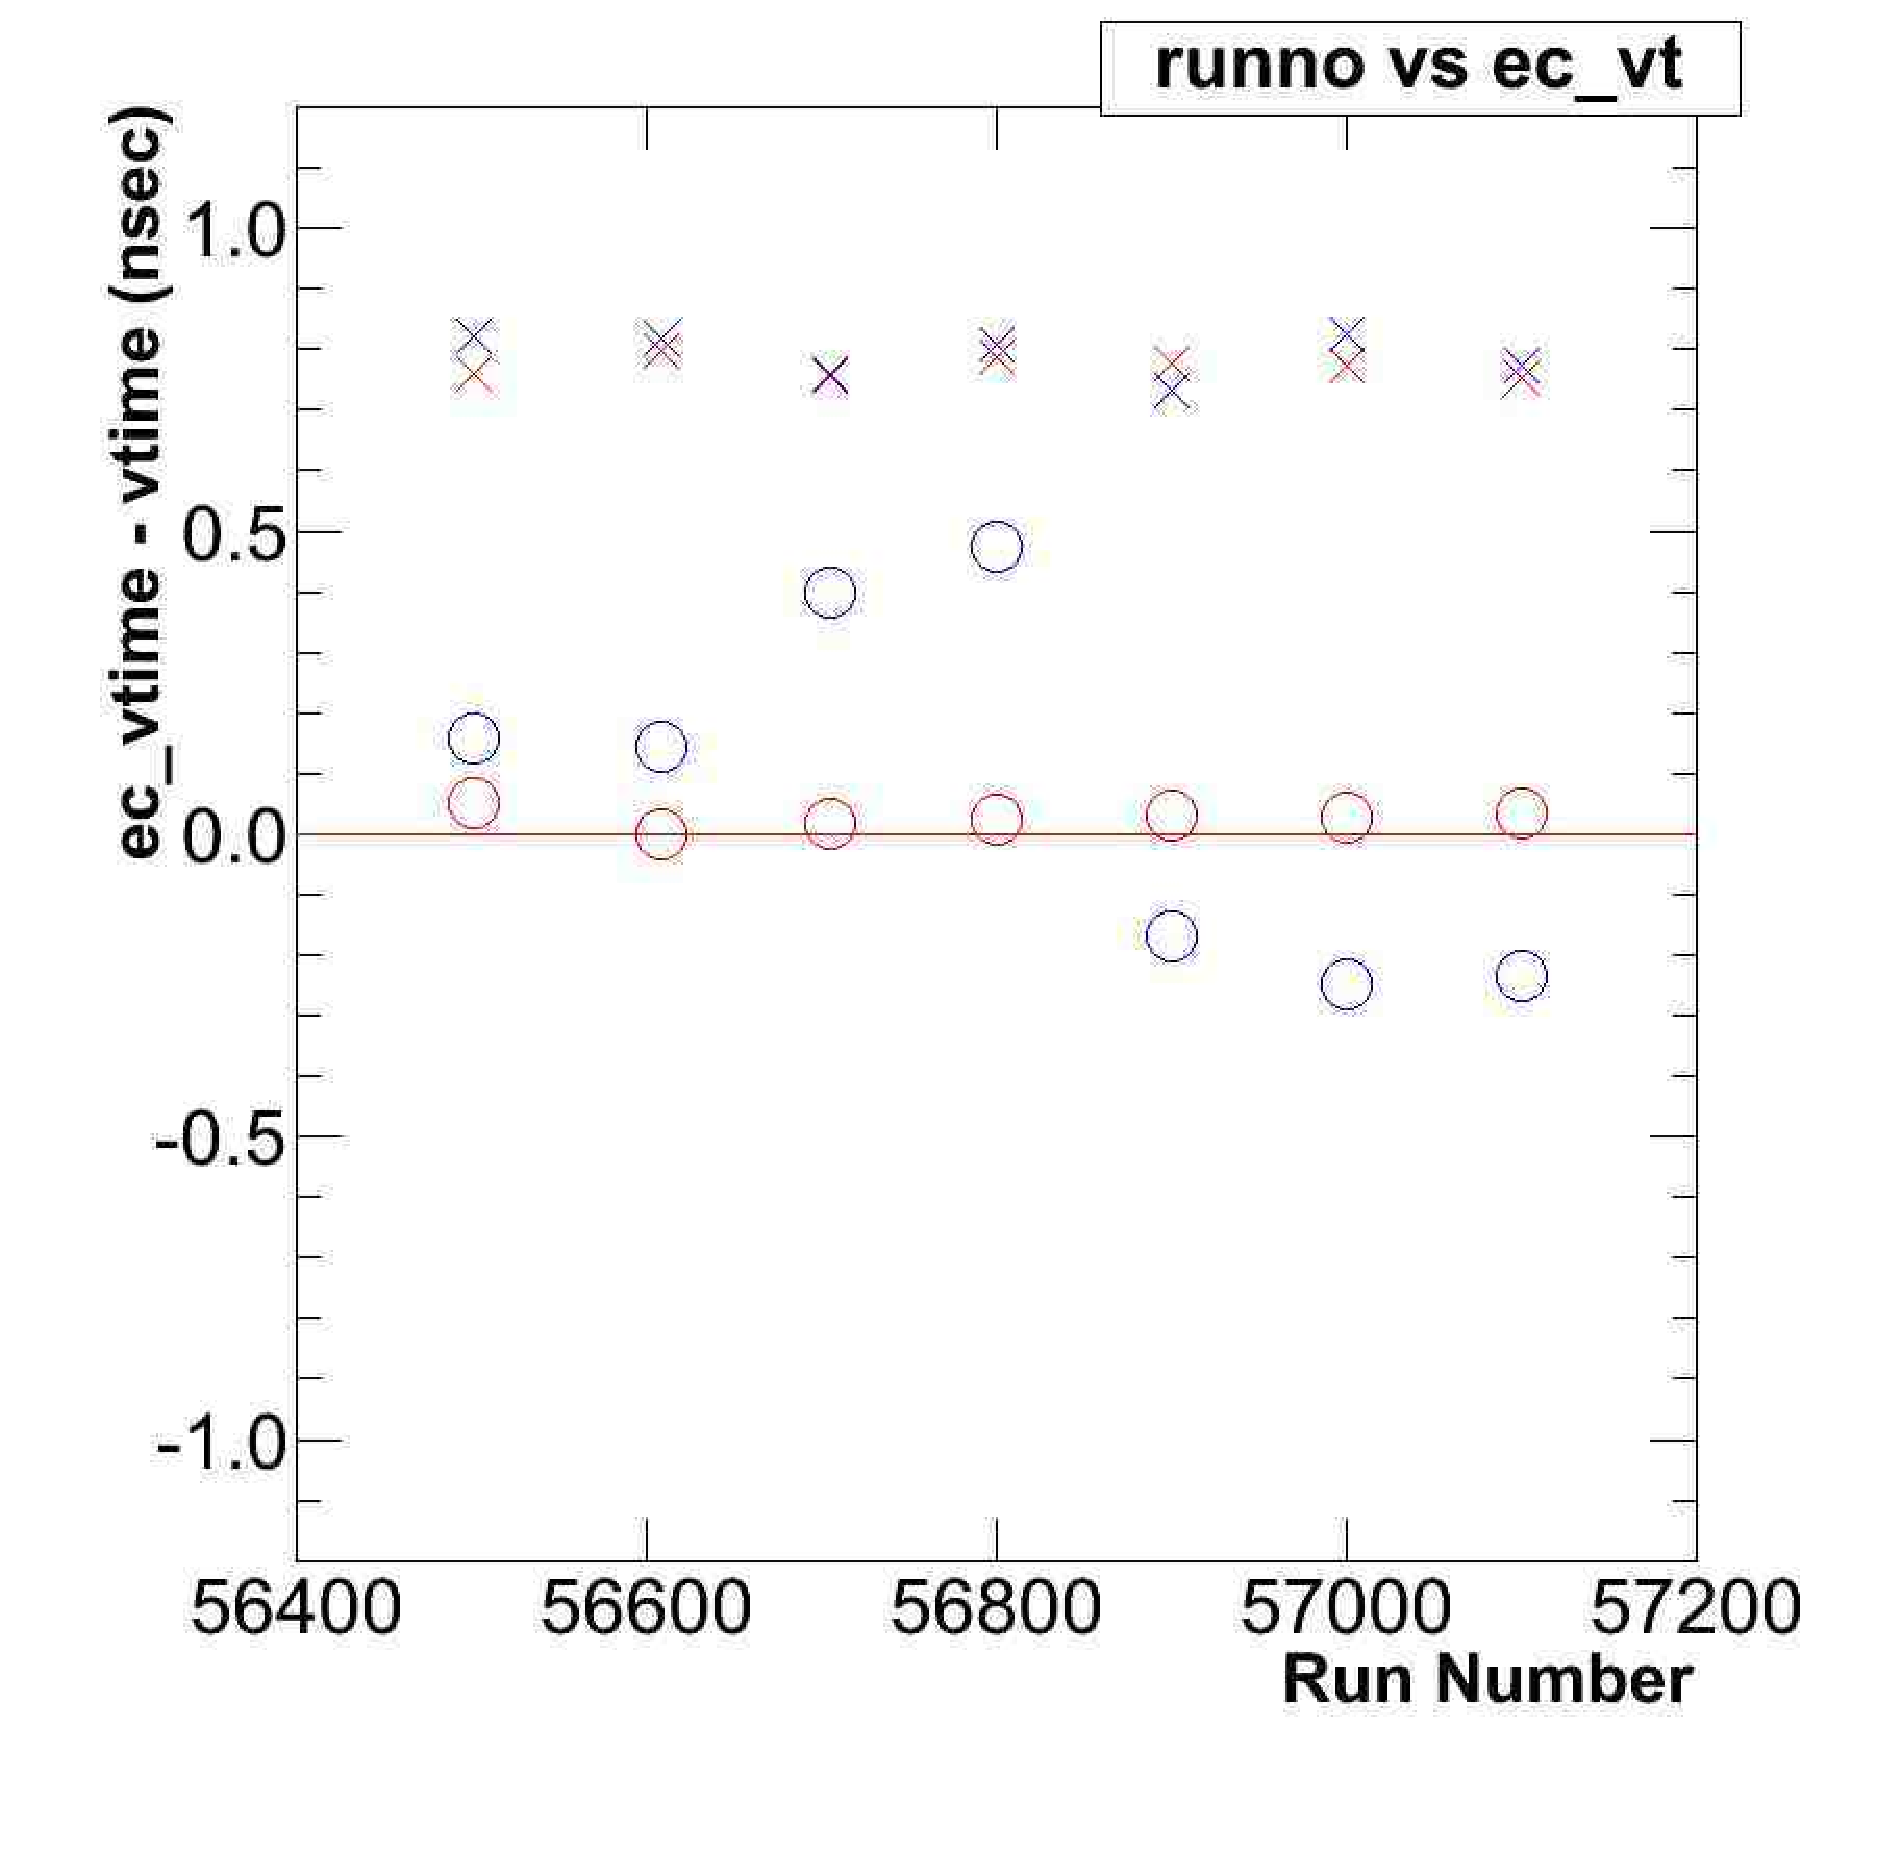
\includegraphics[width=0.45\textwidth]{figures/calib/ec/ec_vtimebyrun.eps}
  \caption{The quality of EC timing calibration, i.e., the mean and $\sigma$ of the photon vertex time according to EC, and the event vertex time, monitored for several run ranges. The ranges are chosen according to Fig.~\ref{ectrunsec}. The inclusion of non-photon backgrounds, in the monitoring process, resulted in a larger value of $\sigma$ than the $500$~ps EC timing resolution shown in Fig.~\ref{etcall}. }
  \label{ectrun}
  \end{center}
\end{figure}

Although not solely dependent on the EC timing calibration quality, the $\pi^0$ mass and resolution are also monitored on a run-by-run basis (Fig.~\ref{ecpi0m}), which shows great stability.

\begin{figure}[h]
\begin{center}
 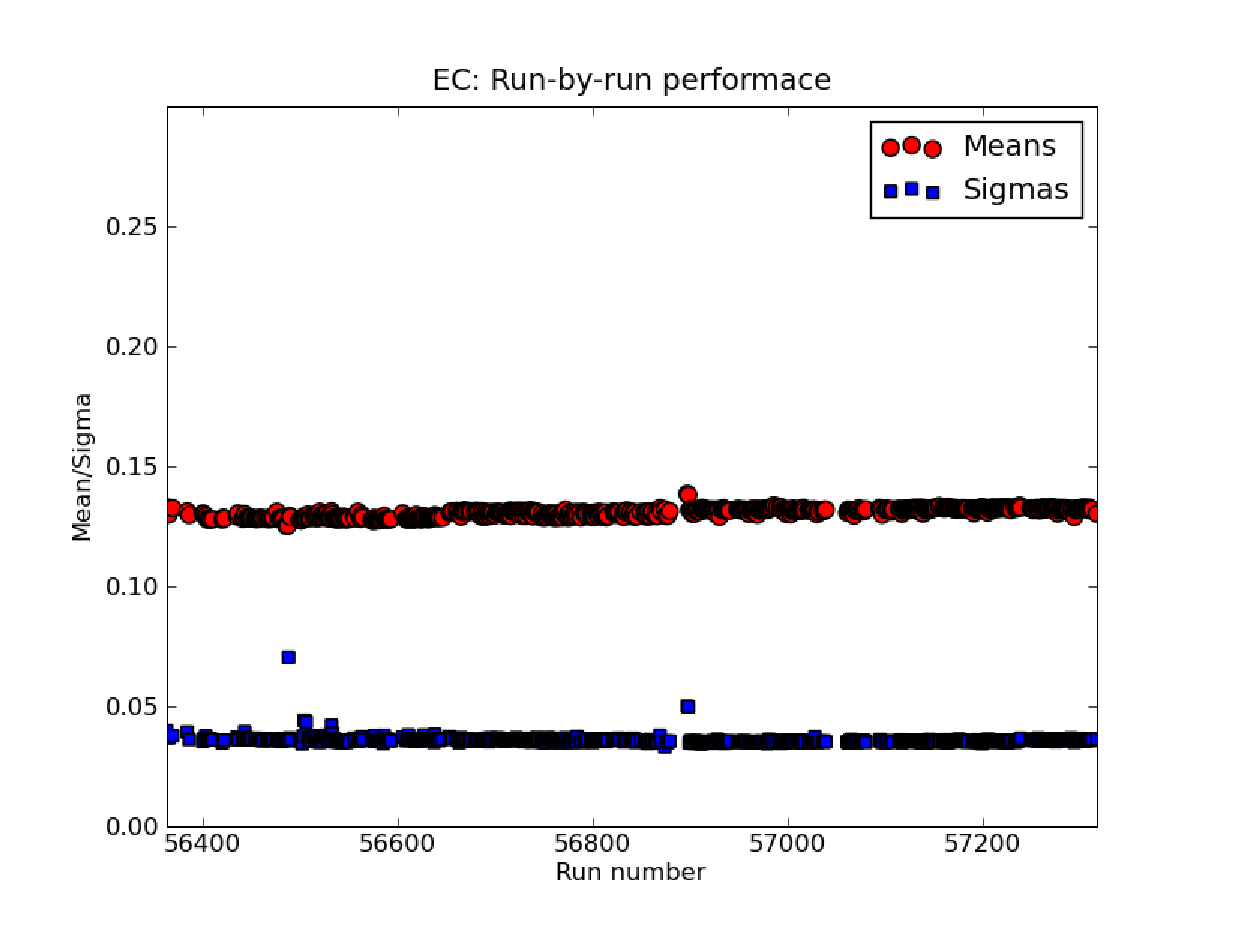
\includegraphics[width=0.45\textwidth]{figures/calib/ec/ec_pi0mass.eps}
  \caption{The mass and resolution of the $\pi^0$, reconstructed from fitting two-photon invariant mass spectra, as a function of the run number.}
  \label{ecpi0m}
  \end{center}
\end{figure}
%
%
%
%
\FloatBarrier
\subsubsection{\label{sec:calib.ec.eff}Electrocalorimeter Efficiency and Bad Paddles}
The efficiency for the \abbr{EC} subsystem is different for each strip in the $u$, $v$, $w$ arrangement. As a result, there are regions of detection which are inefficient. An extreme example of this is illustrated in Fig.~\ref{fig:neg:ec.sec5}, where the \abbr{EC} \emph{inner} (top row) and \emph{outer} (bottom row) strips are plotted as a function of the azimuthal angle~($\phi$) for sector 5. A dead or inefficient strip is seen as a horizontal band in Fig.~\ref{fig:neg:ec.sec5}.  The curvature of inefficient strips seen are reflections of inefficiency in an another orientation. For example, the curves seen in the top left plot, $u$ orientation, of Fig.~\ref{fig:neg:ec.sec5} is a reflection of dead or inefficient strips from $v$ and $w$ orientations respectively.All inefficiencies and cuts shown are for he $e^-$ data. These inefficiencies and cuts are valid for the $e^+$ data.
%
\begin{figure}[h!]\begin{center}
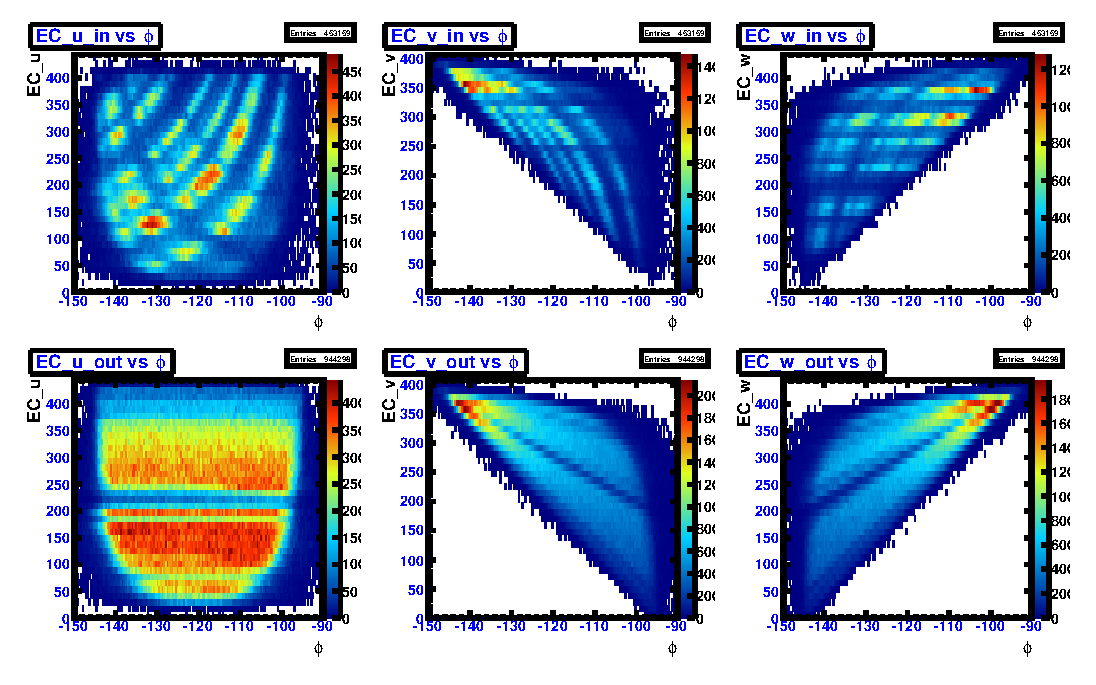
\includegraphics[width=\figwidth,height=\hfigheight]{figures/calib/ec/pim_ecuvw_phi_NOKnockout_sec5.eps}
\caption[Inefficient \abbr{EC} $u$, $v$, $w$ strips vs. $\phi$ for sector 5 in \abbr{CLAS} $e^{-} \ $ data]{\label{fig:neg:ec.sec5}Inefficient \abbr{EC} $u$, $v$, $w$ strips vs. $\phi$ for sector 5 in \abbr{CLAS} $e^{-} \ $ data. Top row depicts the $u$, $v$, $w$ strips for the \emph{inner} \abbr{EC}, while the bottom row depicts the $u$, $v$, $w$ strips for the \emph{outer} \abbr{EC}. The z-axis illustrates the number of hits in the plot. Image source:~\cite{clas.thesis.kunkel}}
\end{center}\end{figure}
%
The projection of Fig.~\ref{fig:neg:ec.sec5} onto the y-axis can be seen in Fig.~\ref{fig:neg.ecstrip.sec5}. This view depicts the actual paddles that are dead or inefficient. It can be seen in either Figs.~\ref{fig:neg:ec.sec5} and~\ref{fig:neg.ecstrip.sec5} that there exists inefficient \abbr{EC} strips for sector 5.
\begin{figure}[h!]\begin{center}
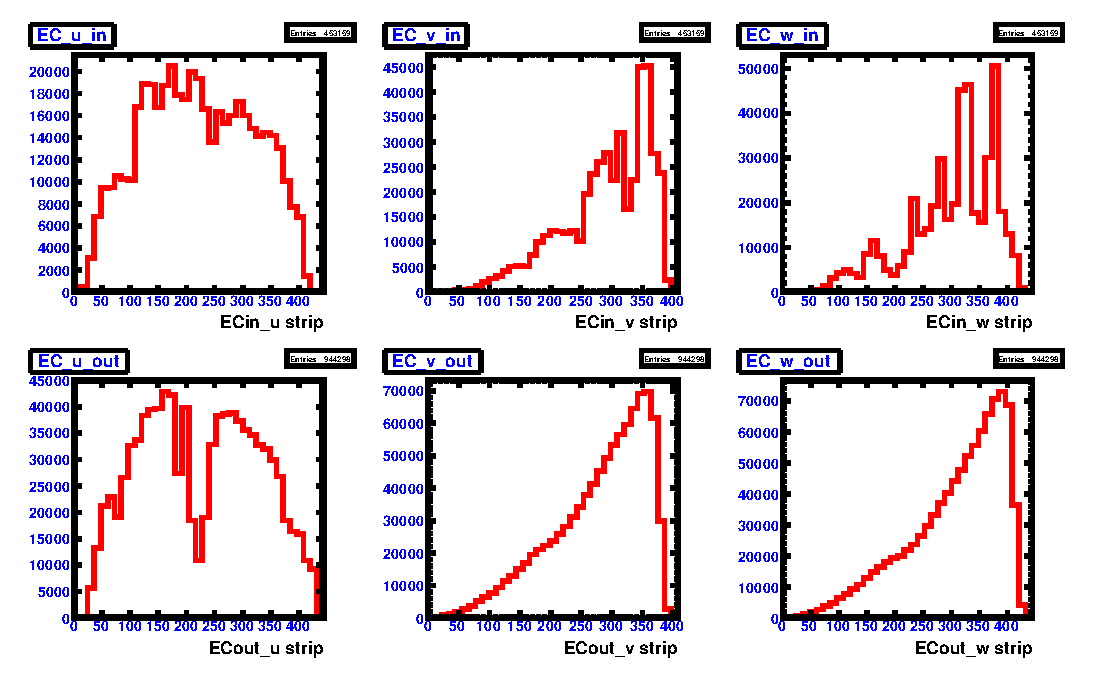
\includegraphics[width=\figwidth,height=\hfigheight]{figures/calib/ec/pim_ecuvw_NOKnockout_sec5.eps}
\caption[Number of hit vs. inefficient \abbr{EC} $u$, $v$, $w$ strips for sector 5 for $e^-$ data]{\label{fig:neg.ecstrip.sec5} Number of hit vs. inefficient \abbr{EC} $u$, $v$, $w$ strips for sector 5 for $e^-$ data. Top row depicts the $u$, $v$, $w$  strips for the \emph{inner} \abbr{EC}, while the bottom row depicts the $u$, $v$, $w$  strips for the \emph{outer} \abbr{EC}. Image source:~\cite{clas.thesis.kunkel}}
\end{center}\end{figure}
The inefficient strips were removed in data and \abbr{MC}. The effect of the inefficient strip cut, along with the standard \abbr{CLAS} \abbr{EC} geometric fiducial cuts can be seen in Fig.~\ref{fig:neg:ec.sec5_cut} and Fig.~\ref{fig:neg.ecstrip.sec5_cut}.
%
\begin{figure}[h!]\begin{center}
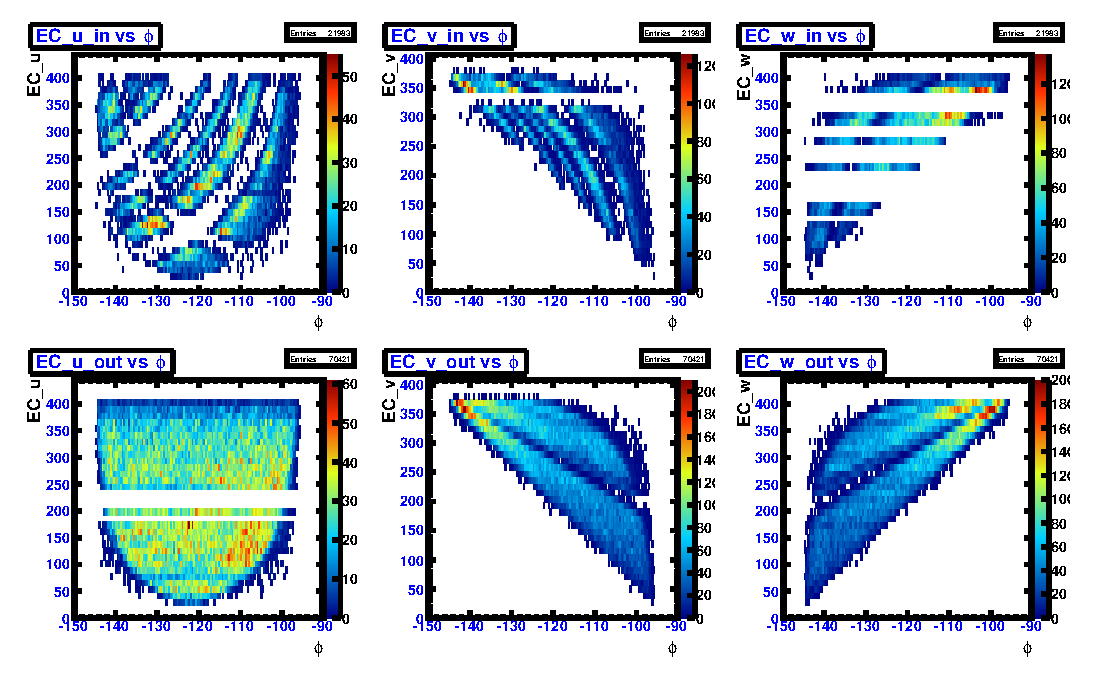
\includegraphics[width=\figwidth,height=\hfigheight]{figures/calib/ec/pim_ecuvw_phi_afterGeoFid_sec5.eps}
\caption[\abbr{EC} $u$, $v$, $w$ strips vs. $\phi$ for sector 5 with fiducial cuts and inefficient paddle knockouts applied to $e^-$ data]{\label{fig:neg:ec.sec5_cut} \abbr{EC} $u$, $v$, $w$ strips vs. $\phi$ for sector 5 with fiducial cuts and inefficient paddle knockouts applied to $e^-$ data. Top row depicts the $u$, $v$, $w$ strips for the \emph{inner} \abbr{EC}, while the bottom row depicts the $u$, $v$, $w$ strips for the \emph{outer} \abbr{EC}. The z-axis illustrates the number of hits in the plot. Image source:~\cite{clas.thesis.kunkel}}
\end{center}\end{figure}
%
\begin{figure}[h!]\begin{center}
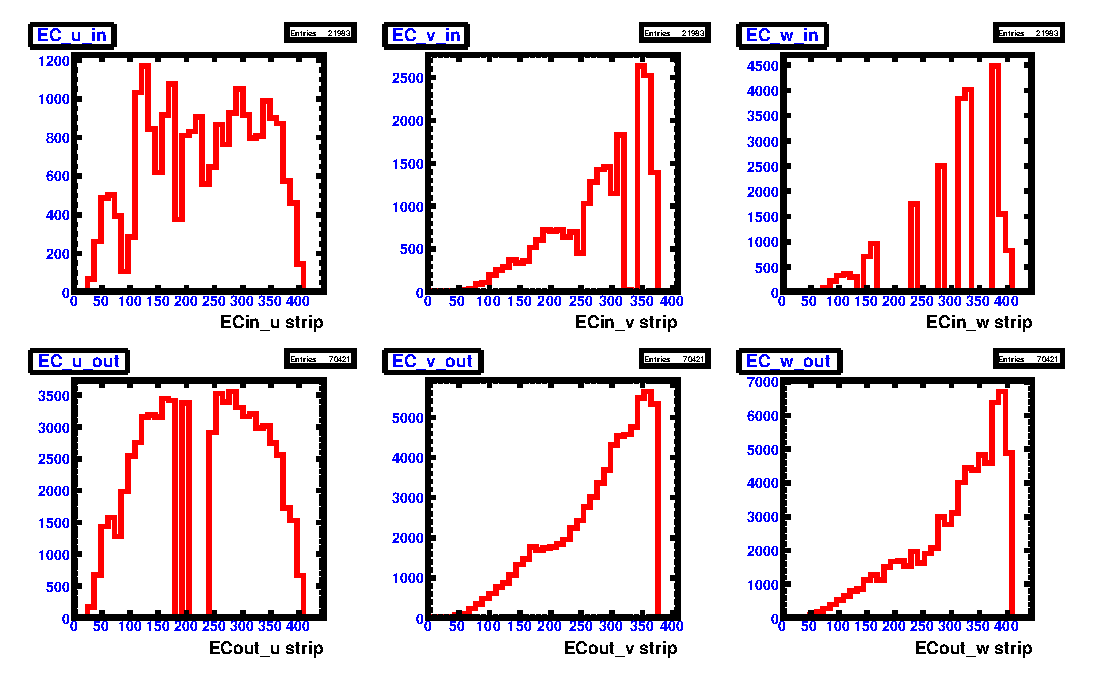
\includegraphics[width=\figwidth,height=\hfigheight]{figures/calib/ec/pim_ecuvw_afterGeoFid_sec5.eps}
\caption[Number of hits vs. \abbr{EC} $u$, $v$, $w$ strips for sector 5 with fiducial cuts and inefficient paddle knockouts applied to $e^-$ data]{\label{fig:neg.ecstrip.sec5_cut}Number of hits vs. \abbr{EC} $u$, $v$, $w$ strips for sector 5 with fiducial cuts and inefficient paddle knockouts applied to $e^-$ data. Top row depicts the $u$, $v$, $w$ strips for the \emph{inner} \abbr{EC}, while the bottom row depicts the $u$, $v$, $w$ strips for the \emph{outer} \abbr{EC}. Image source:~\cite{clas.thesis.kunkel}}
\end{center}\end{figure}
\FloatBarrier
The inefficiencies for the other 5 sectors are
% % % %SECTOR 1
\begin{figure}[!ht]
  \centering
  \begin{subfigure}[b]{\figwidth}
  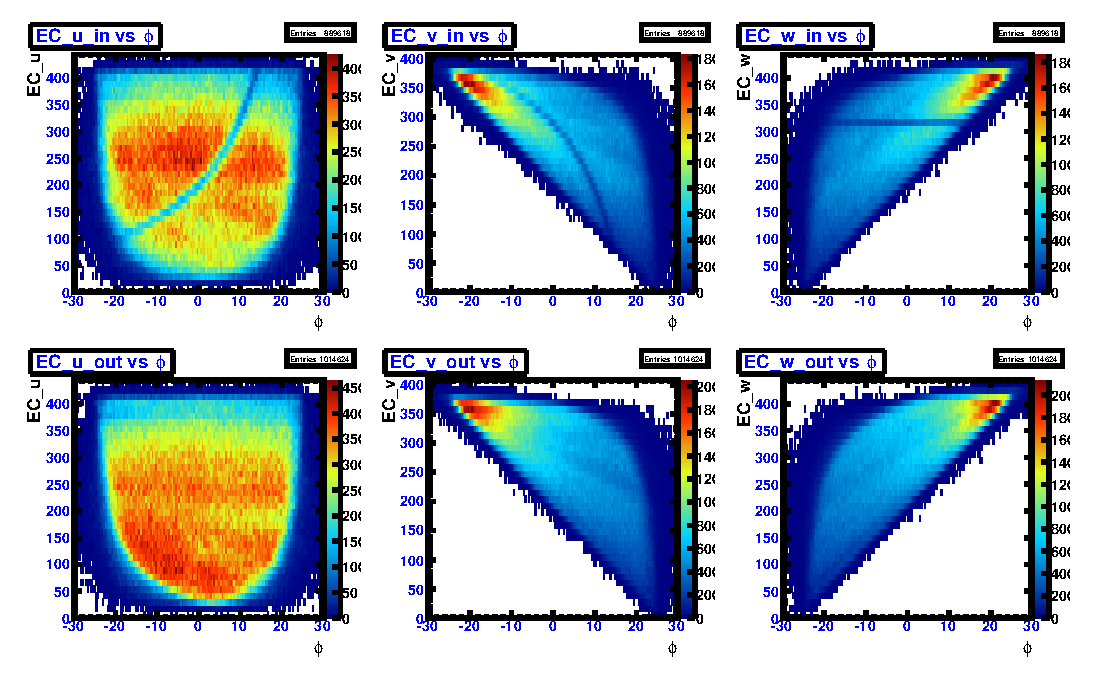
\includegraphics[width=\figwidth, height=3.5in,valign=c]{figures/calib/ec/pim_ecuvw_phi_NOKnockout_sec1.eps}\caption{}\label{fig:EC_I_I}
  \end{subfigure}%
  \\
  \begin{subfigure}[b]{\figwidth}
  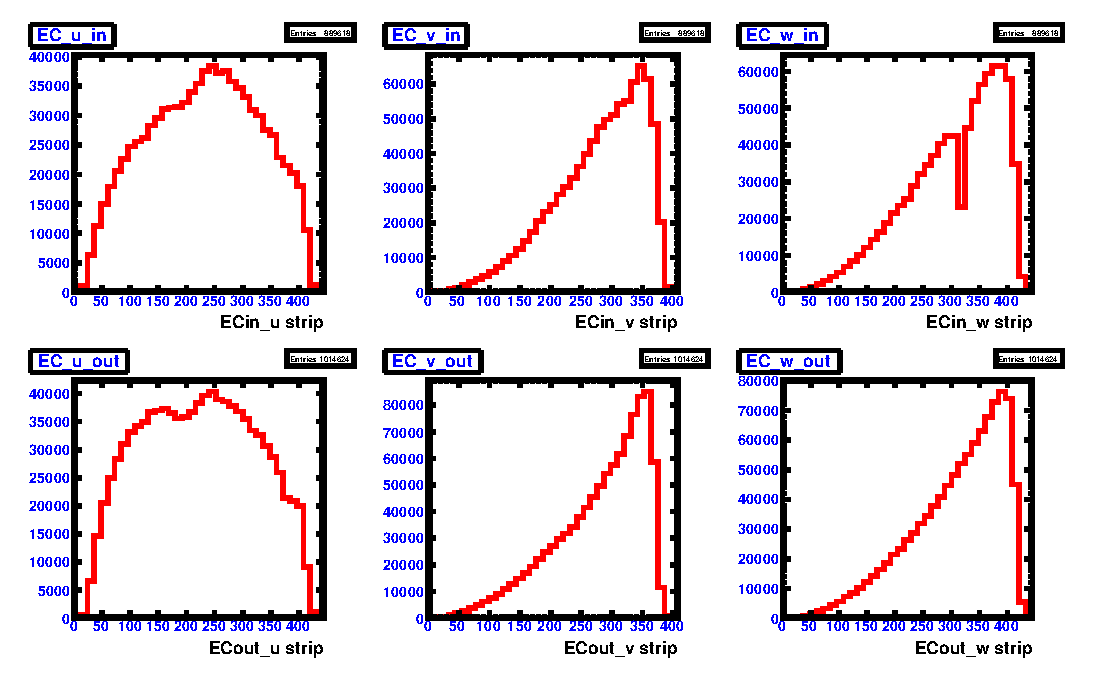
\includegraphics[width=\figwidth, height=3.5in,valign=c]{figures/calib/ec/pim_ecuvw_NOKnockout_sec1.eps}\caption{}\label{fig:EC_II_I}
  \end{subfigure}%
      \caption {Inefficient \abbr{EC} $u$, $v$, $w$ strips vs. $\phi$ for sector 1 in \abbr{CLAS} $e^{-} \ $ data~(\subref{fig:EC_I_I}), notation the same as Fig.~\ref{fig:neg:ec.sec5}. Number of hits vs. inefficient \abbr{EC} $u$, $v$, $w$ strips for sector 1 for $e^-$ data~(\subref{fig:EC_II_I}). Notation same as in Fig.~\ref{fig:neg.ecstrip.sec5}. Image source:~\cite{clas.thesis.kunkel}}
        \label{fig:EC_no_I}
\end{figure}



\begin{figure}[!ht]
  \centering
  \begin{subfigure}[b]{\figwidth}
  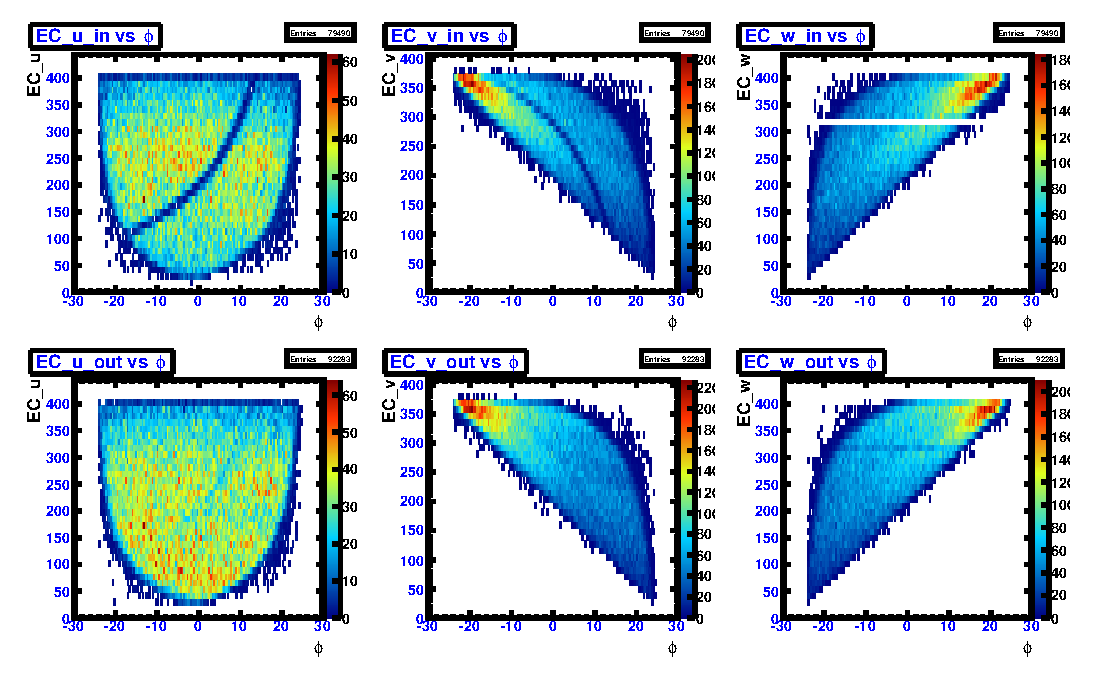
\includegraphics[width=\figwidth, height=3.5in,valign=c]{figures/calib/ec/pim_ecuvw_phi_afterGeoFid_sec1.eps}\caption{}\label{fig:EC_III_I}
  \end{subfigure}%
  \\
  \begin{subfigure}[b]{\figwidth}
  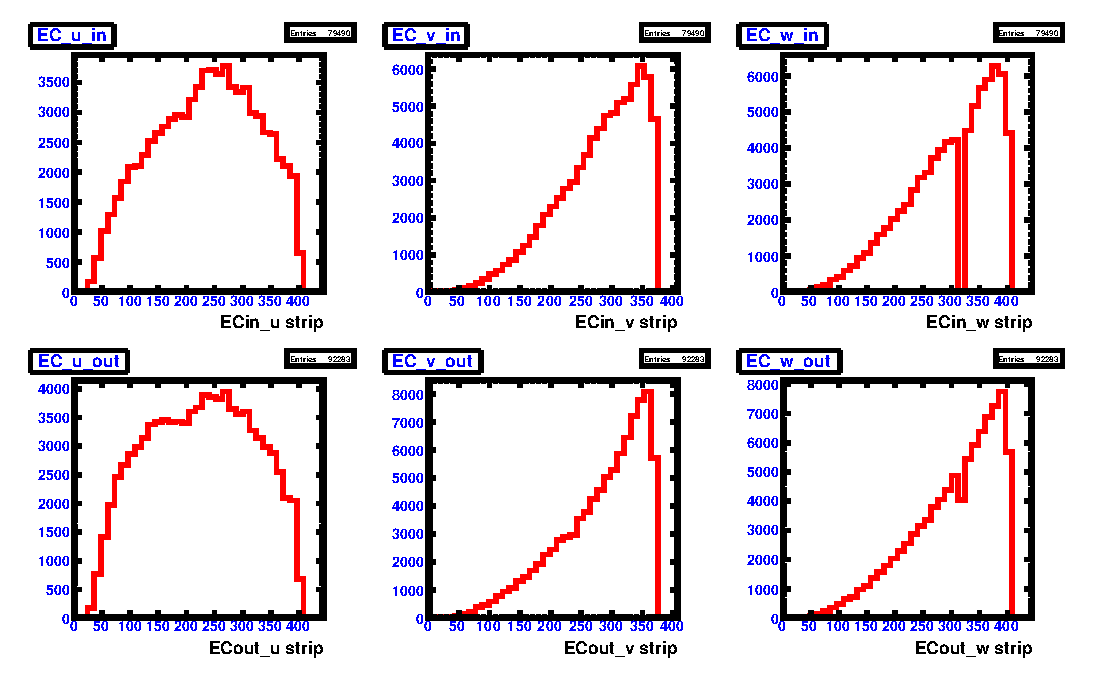
\includegraphics[width=\figwidth, height=3.5in,valign=c]{figures/calib/ec/pim_ecuvw_afterGeoFid_sec1.eps}\caption{}\label{fig:EC_IV_I}
  \end{subfigure}%
      \caption {\abbr{EC} $u$, $v$, $w$ strips vs. $\phi$ for sector 1 with fiducial cuts and inefficient paddle knockouts applied to $e^-$ data~(\ref{fig:EC_III_I}), notation the same as Fig.~\ref{fig:neg:ec.sec5_cut}. Number of hits vs. \abbr{EC} $u$, $v$, $w$ strips for sector 1 with fiducial cuts and inefficient paddle knockouts applied to $e^-$ data~(\ref{fig:EC_IV_I}). Notation same as in Fig.~\ref{fig:neg.ecstrip.sec5_cut}. Image source:~\cite{clas.thesis.kunkel}}
        \label{fig:EC_cut_I}
\end{figure}


%% % % %SECTOR 2
\begin{figure}[!ht]
  \centering
  \begin{subfigure}[b]{\figwidth}
  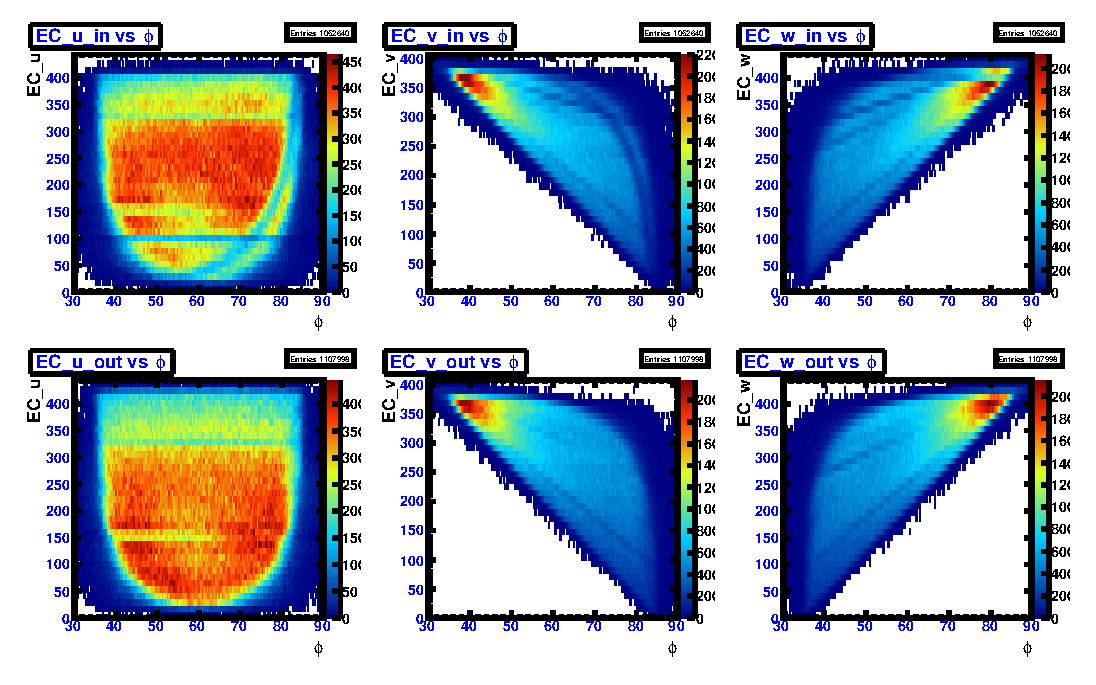
\includegraphics[width=\figwidth, height=3.5in,valign=c]{figures/calib/ec/pim_ecuvw_phi_NOKnockout_sec2.eps}\caption{}\label{fig:EC_I_II}
  \end{subfigure}%
  \\
  \begin{subfigure}[b]{\figwidth}
  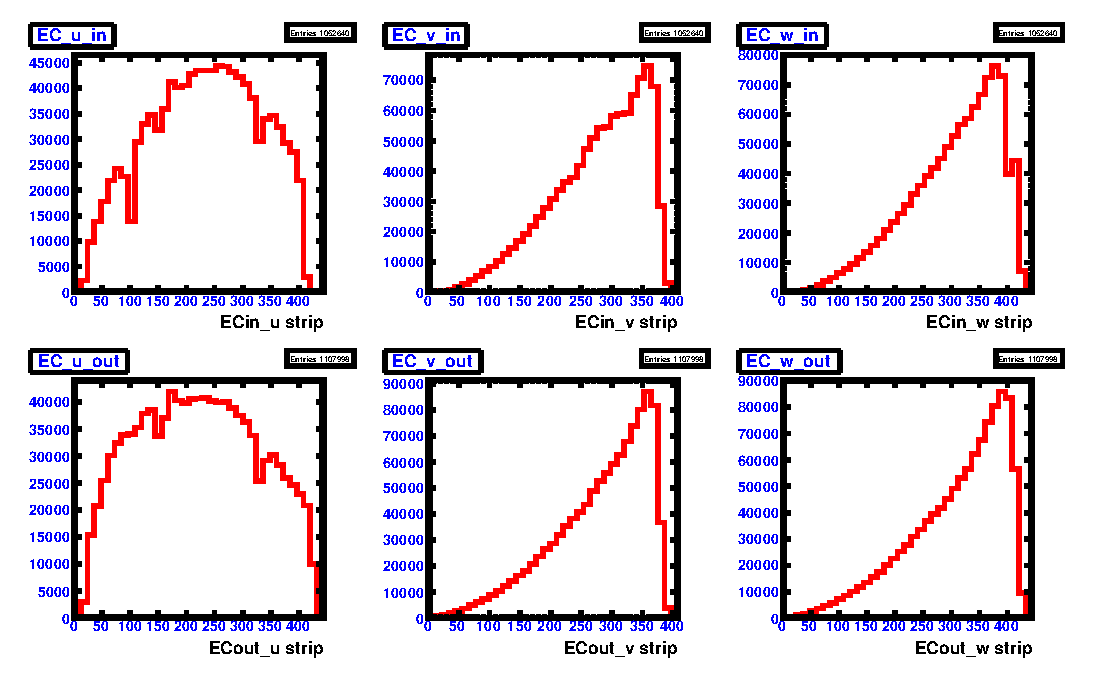
\includegraphics[width=\figwidth, height=3.5in,valign=c]{figures/calib/ec/pim_ecuvw_NOKnockout_sec2.eps}\caption{}\label{fig:EC_II_II}
  \end{subfigure}%
      \caption {Inefficient \abbr{EC} $u$, $v$, $w$ strips vs. $\phi$ for sector 2 in \abbr{CLAS} $e^{-} \ $ data~(\ref{fig:EC_I_II}), notation the same as Fig.~\ref{fig:neg:ec.sec5}. Number of hits vs. inefficient \abbr{EC} $u$, $v$, $w$ strips for sector 2 for $e^-$ data~(\ref{fig:EC_II_II}). Notation same as in Fig.~\ref{fig:neg.ecstrip.sec5}. Image source:~\cite{clas.thesis.kunkel}}
        \label{fig:EC_no_II}
\end{figure}



\begin{figure}[!ht]
  \centering
  \begin{subfigure}[b]{\figwidth}
  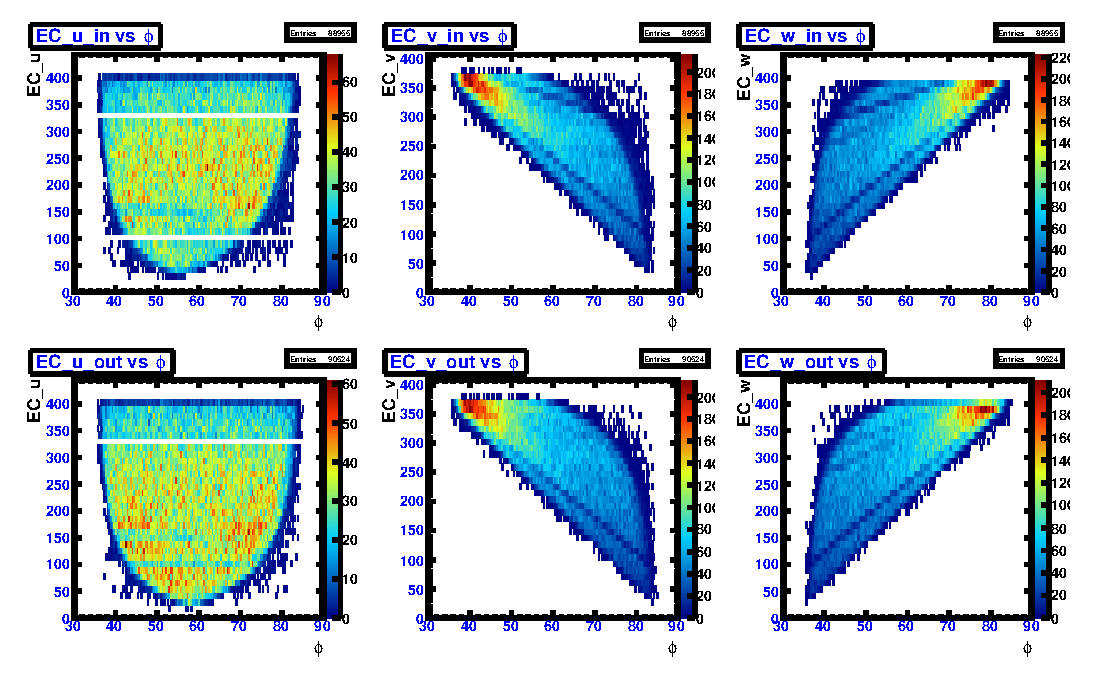
\includegraphics[width=\figwidth, height=3.5in,valign=c]{figures/calib/ec/pim_ecuvw_phi_afterGeoFid_sec2.eps}\caption{}\label{fig:EC_III_II}
  \end{subfigure}%
  \\
  \begin{subfigure}[b]{\figwidth}
  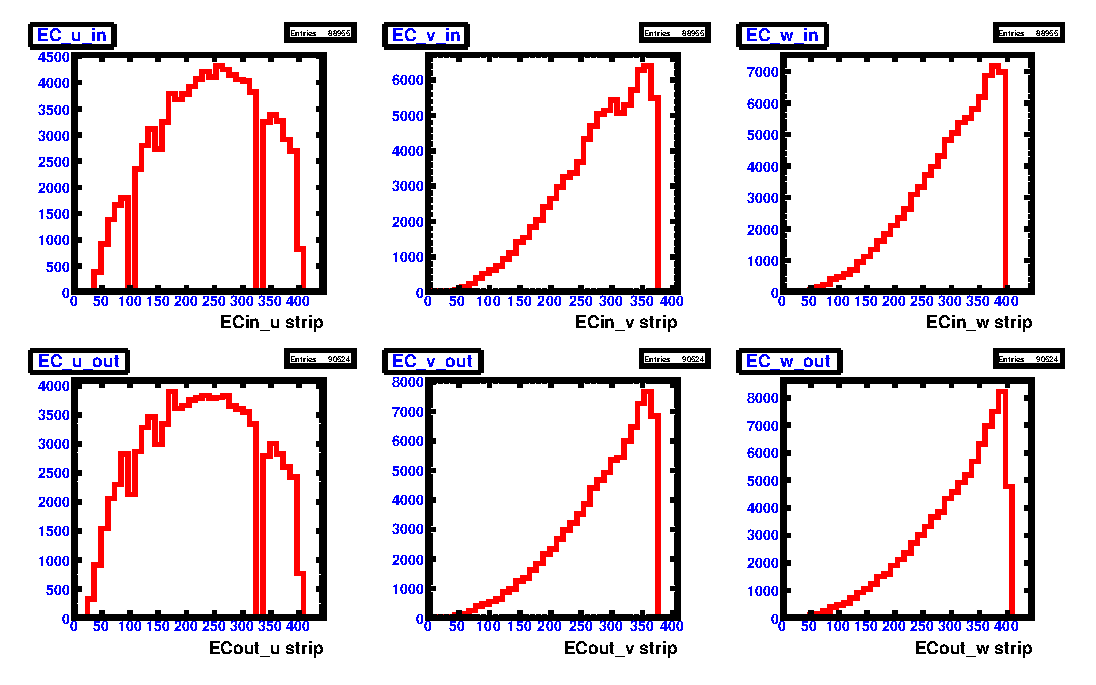
\includegraphics[width=\figwidth, height=3.5in,valign=c]{figures/calib/ec/pim_ecuvw_afterGeoFid_sec2.eps}\caption{}\label{fig:EC_IV_II}
  \end{subfigure}%
      \caption {\abbr{EC} $u$, $v$, $w$ strips vs. $\phi$ for sector 2 with fiducial cuts and inefficient paddle knockouts applied to $e^-$ data~(\ref{fig:EC_III_II}), notation the same as Fig.~\ref{fig:neg:ec.sec5_cut}. Number of hits vs. \abbr{EC} $u$, $v$, $w$ strips for sector 2 with fiducial cuts and inefficient paddle knockouts applied to $e^-$ data~(\ref{fig:EC_IV_II}). Notation same as in Fig.~\ref{fig:neg.ecstrip.sec5_cut}. Image source:~\cite{clas.thesis.kunkel}}
        \label{fig:EC_cut_II}
\end{figure}

%
%% % % %SECTOR 3
\begin{figure}[!ht]
  \centering
  \begin{subfigure}[b]{\figwidth}
  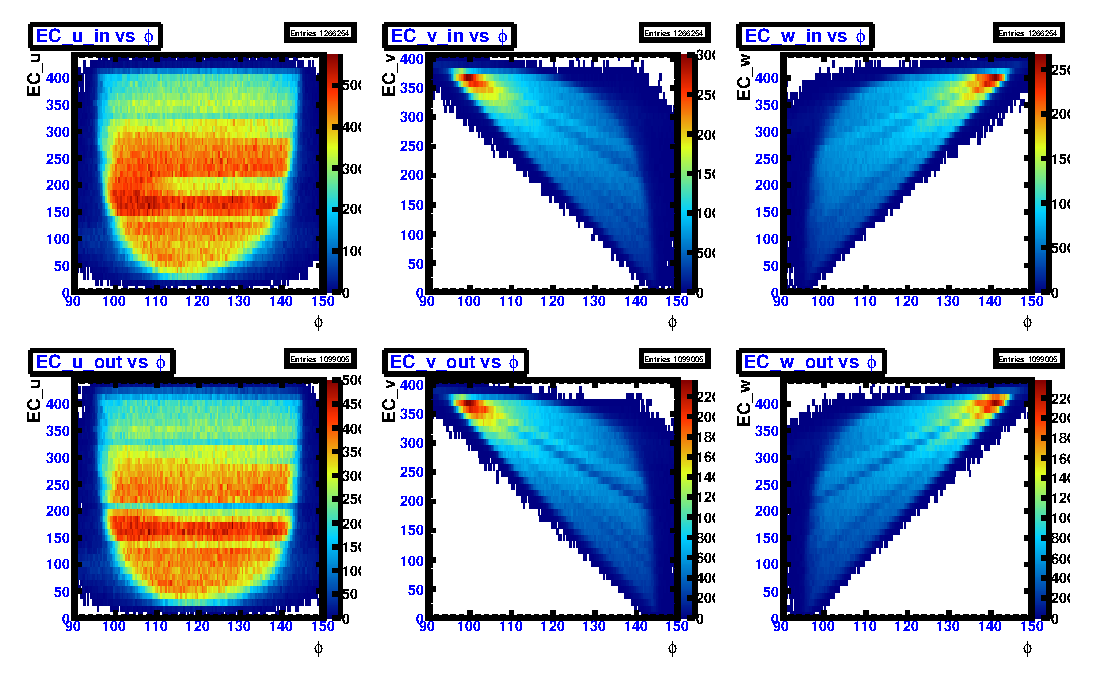
\includegraphics[width=\figwidth, height=3.5in,valign=c]{figures/calib/ec/pim_ecuvw_phi_NOKnockout_sec3.eps}\caption{}\label{fig:EC_I_III}
  \end{subfigure}%
  \\
  \begin{subfigure}[b]{\figwidth}
  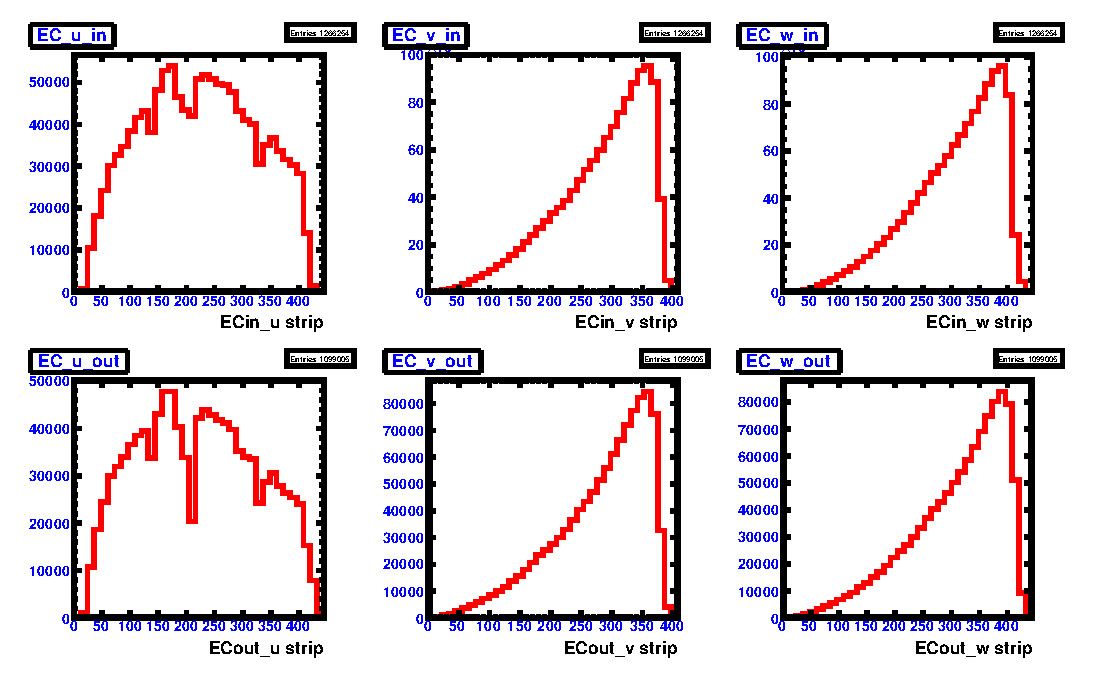
\includegraphics[width=\figwidth, height=3.5in,valign=c]{figures/calib/ec/pim_ecuvw_NOKnockout_sec3.eps}\caption{}\label{fig:EC_II_III}
  \end{subfigure}%
      \caption {Inefficient \abbr{EC} $u$, $v$, $w$ strips vs. $\phi$ for sector 3 in \abbr{CLAS} $e^{-} \ $ data~(\ref{fig:EC_I_III}), notation the same as Fig.~\ref{fig:neg:ec.sec5}. Number of hits vs. inefficient \abbr{EC} $u$, $v$, $w$ strips for sector 3 for $e^-$ data~(\ref{fig:EC_II_III}). Notation same as in Fig.~\ref{fig:neg.ecstrip.sec5}. Image source:~\cite{clas.thesis.kunkel}}
        \label{fig:EC_no_III}
\end{figure}



\begin{figure}[!ht]
  \centering
  \begin{subfigure}[b]{\figwidth}
  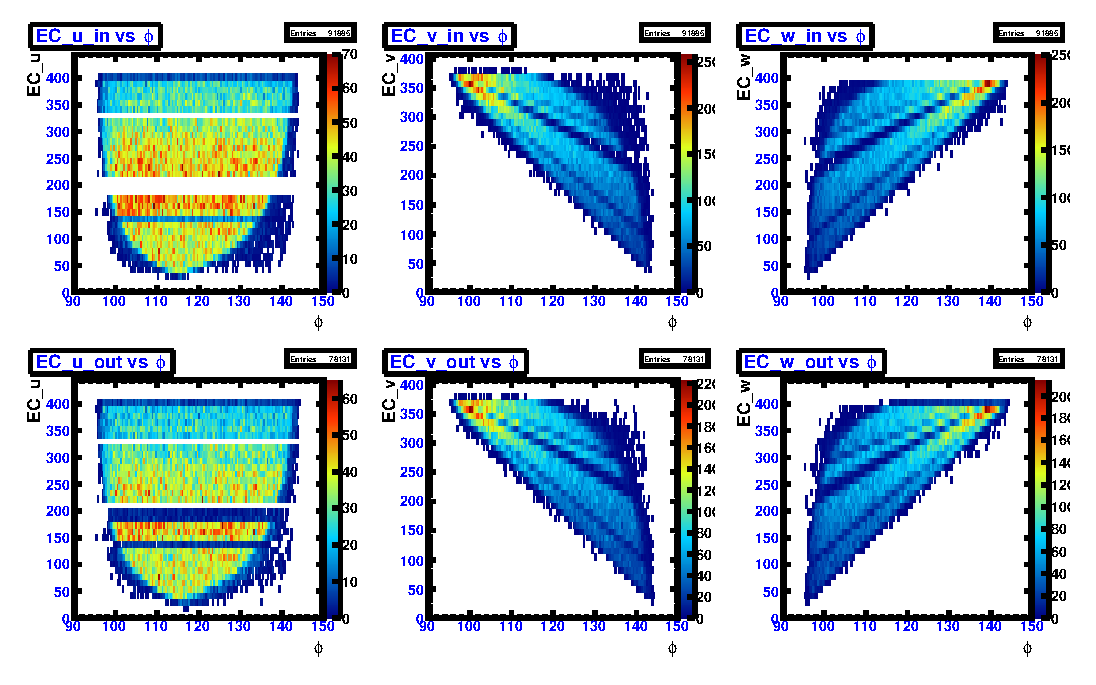
\includegraphics[width=\figwidth, height=3.5in,valign=c]{figures/calib/ec/pim_ecuvw_phi_afterGeoFid_sec3.eps}\caption{}\label{fig:EC_III_III}
  \end{subfigure}%
  \\
  \begin{subfigure}[b]{\figwidth}
  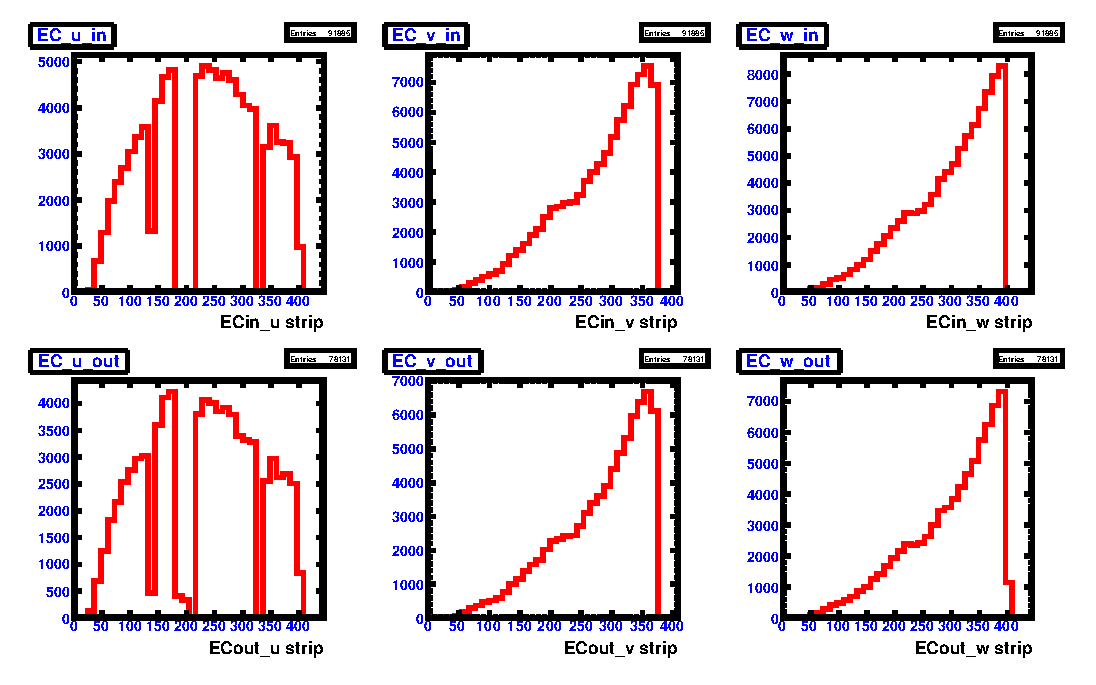
\includegraphics[width=\figwidth, height=3.5in,valign=c]{figures/calib/ec/pim_ecuvw_afterGeoFid_sec3.eps}\caption{}\label{fig:EC_IV_III}
  \end{subfigure}%
      \caption {\abbr{EC} $u$, $v$, $w$ strips vs. $\phi$ for sector 3 with fiducial cuts and inefficient paddle knockouts applied to $e^-$ data~(\ref{fig:EC_III_III}), notation the same as Fig.~\ref{fig:neg:ec.sec5_cut}. Number of hits vs. \abbr{EC} $u$, $v$, $w$ strips for sector 3 with fiducial cuts and inefficient paddle knockouts applied to $e^-$ data~(\ref{fig:EC_IV_III}). Notation same as in Fig.~\ref{fig:neg.ecstrip.sec5_cut}. Image source:~\cite{clas.thesis.kunkel}}
        \label{fig:EC_cut_III}
\end{figure}


%% % % %SECTOR 4
\begin{figure}[!ht]
  \centering
  \begin{subfigure}[b]{\figwidth}
  \includegraphics[width=\figwidth, height=3.5in,valign=c]{figures/calib/ec/pim_ecuvw_phi_NOKnockout_sec4.eps}\caption{}\label{fig:EC_I_IV}
  \end{subfigure}%
  \\
  \begin{subfigure}[b]{\figwidth}
  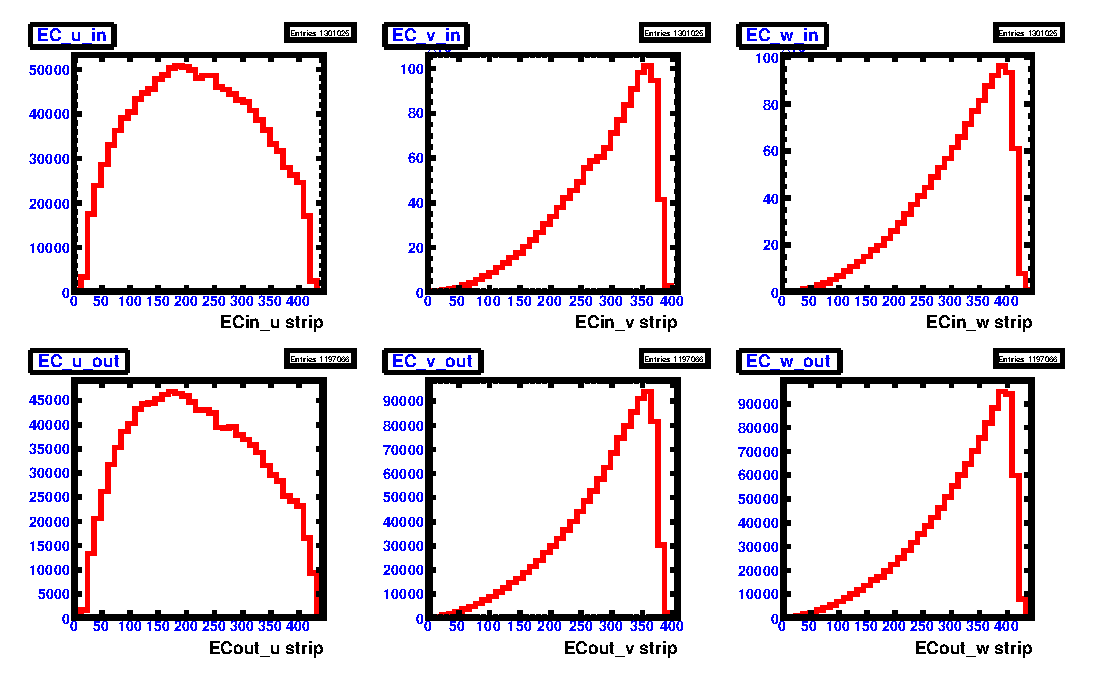
\includegraphics[width=\figwidth, height=3.5in,valign=c]{figures/calib/ec/pim_ecuvw_NOKnockout_sec4.eps}\caption{}\label{fig:EC_II_IV}
  \end{subfigure}%
      \caption {Inefficient \abbr{EC} $u$, $v$, $w$ strips vs. $\phi$ for sector 4 in \abbr{CLAS} $e^{-} \ $ data~(\ref{fig:EC_I_IV}), notation the same as Fig.~\ref{fig:neg:ec.sec5}. Number of hits vs. inefficient \abbr{EC} $u$, $v$, $w$ strips for sector 4 for $e^-$ data~(\ref{fig:EC_II_IV}). Notation same as in Fig.~\ref{fig:neg.ecstrip.sec5}. Image source:~\cite{clas.thesis.kunkel}}
        \label{fig:EC_no_IV}
\end{figure}



\begin{figure}[!ht]
  \centering
  \begin{subfigure}[b]{\figwidth}
  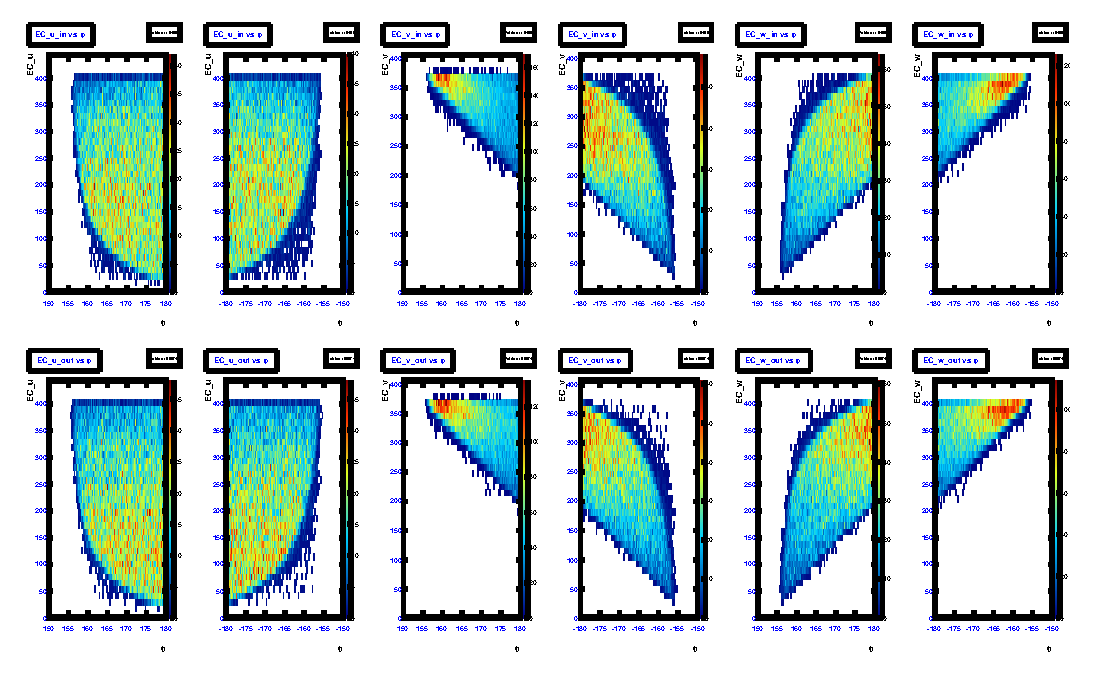
\includegraphics[width=\figwidth, height=3.5in,valign=c]{figures/calib/ec/pim_ecuvw_phi_afterGeoFid_sec4.eps}\caption{}\label{fig:EC_III_IV}
  \end{subfigure}%
  \\
  \begin{subfigure}[b]{\figwidth}
  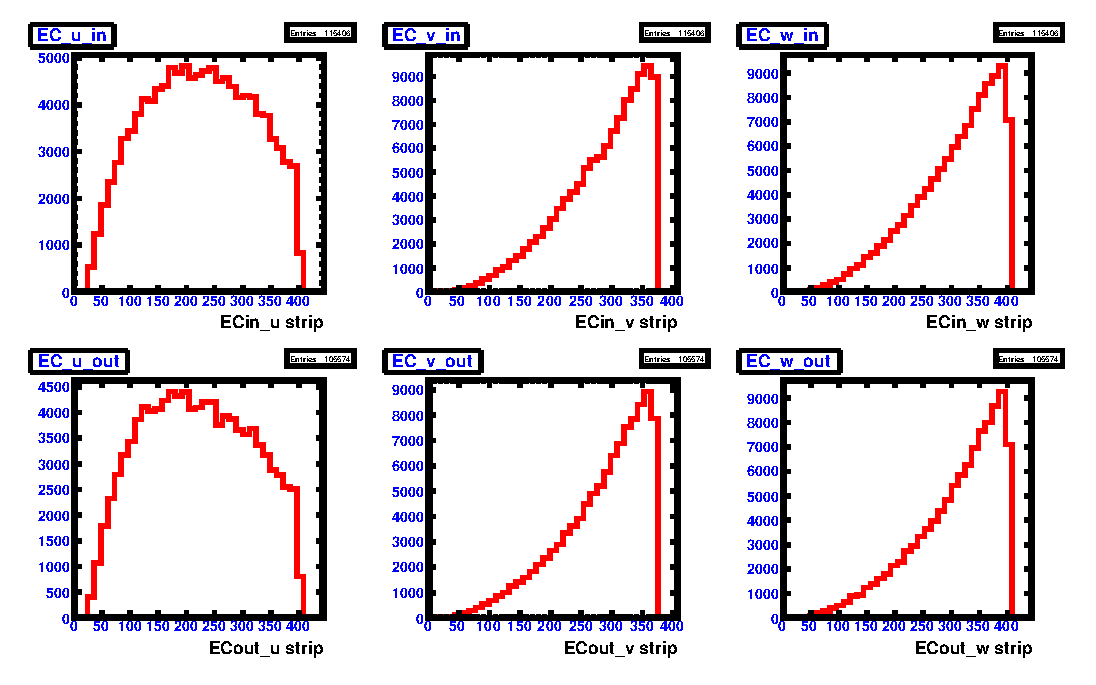
\includegraphics[width=\figwidth, height=3.5in,valign=c]{figures/calib/ec/pim_ecuvw_afterGeoFid_sec4.eps}\caption{}\label{fig:EC_IV_IV}
  \end{subfigure}%
      \caption {\abbr{EC} $u$, $v$, $w$ strips vs. $\phi$ for sector 4 with fiducial cuts and inefficient paddle knockouts applied to $e^-$ data~(\ref{fig:EC_III_IV}), notation the same as Fig.~\ref{fig:neg:ec.sec5_cut}. Number of hits vs. \abbr{EC} $u$, $v$, $w$ strips for sector 4 with fiducial cuts and inefficient paddle knockouts applied to $e^-$ data~(\ref{fig:EC_IV_IV}). Notation same as in Fig.~\ref{fig:neg.ecstrip.sec5_cut}. Image source:~\cite{clas.thesis.kunkel}}
        \label{fig:EC_cut_IV}
\end{figure}


% % % %SECTOR 6
\begin{figure}[!ht]
  \centering
  \begin{subfigure}[b]{\figwidth}
  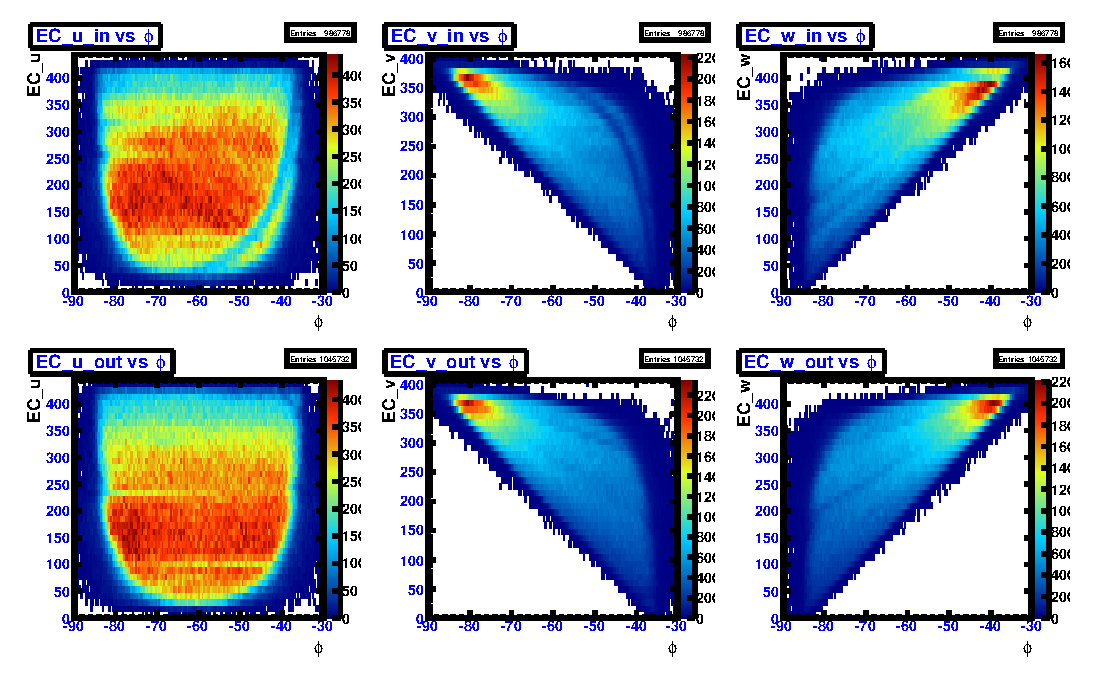
\includegraphics[width=\figwidth, height=3.5in,valign=c]{figures/calib/ec/pim_ecuvw_phi_NOKnockout_sec6.eps}\caption{}\label{fig:EC_I_VI}
  \end{subfigure}%
  \\
  \begin{subfigure}[b]{\figwidth}
  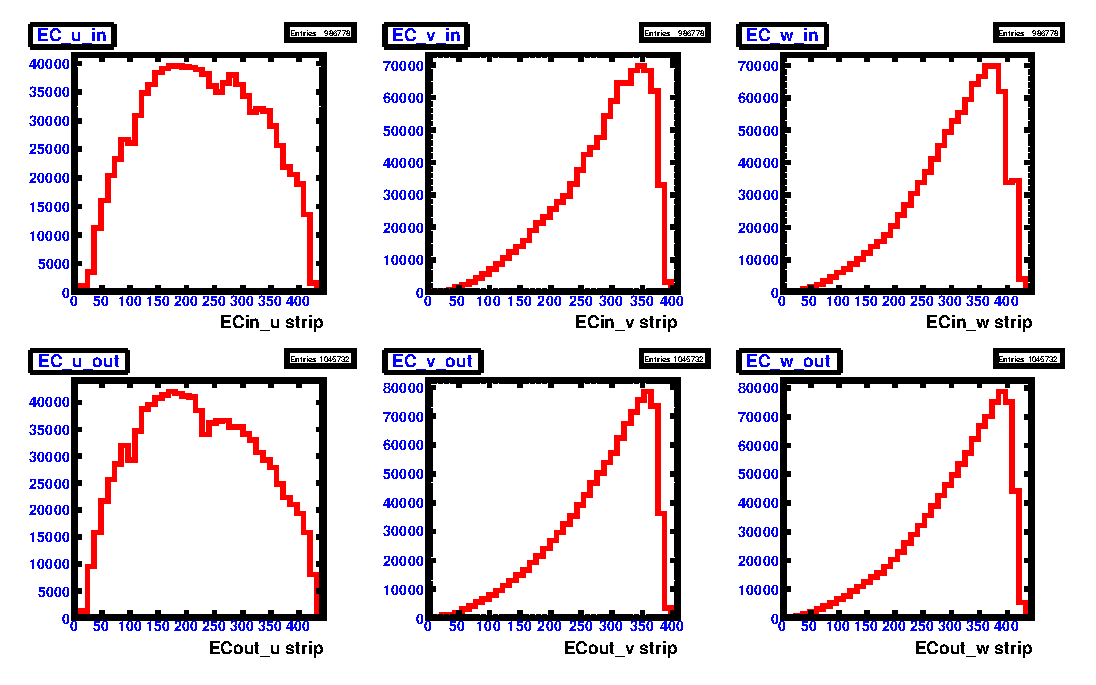
\includegraphics[width=\figwidth, height=3.5in,valign=c]{figures/calib/ec/pim_ecuvw_NOKnockout_sec6.eps}\caption{}\label{fig:EC_II_VI}
  \end{subfigure}%
      \caption {Inefficient \abbr{EC} $u$, $v$, $w$ strips vs. $\phi$ for sector 6 in \abbr{CLAS} $e^{-} \ $ data~(\ref{fig:EC_I_VI}), notation the same as Fig.~\ref{fig:neg:ec.sec5}. Number of hits vs. inefficient \abbr{EC} $u$, $v$, $w$ strips for sector 6 for $e^-$ data~(\ref{fig:EC_II_VI}). Notation same as in Fig.~\ref{fig:neg.ecstrip.sec5}. Image source:~\cite{clas.thesis.kunkel}}
        \label{fig:EC_no_VI}
\end{figure}



\begin{figure}[!ht]
  \centering
  \begin{subfigure}[b]{\figwidth}
  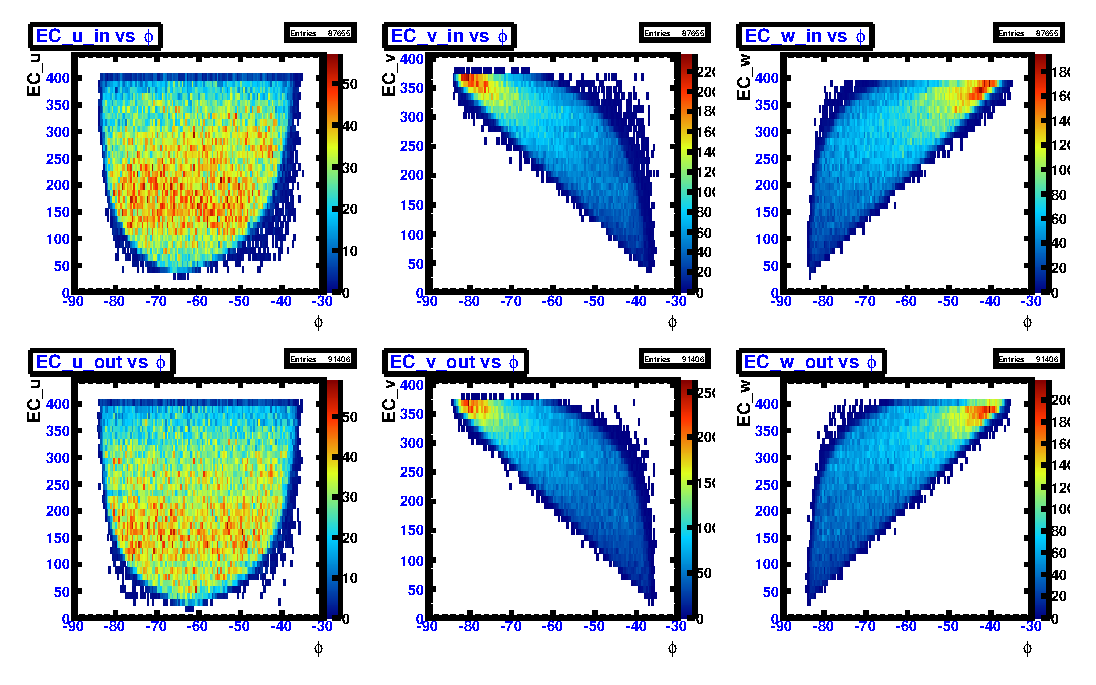
\includegraphics[width=\figwidth, height=3.5in,valign=c]{figures/calib/ec/pim_ecuvw_phi_afterGeoFid_sec6.eps}\caption{}\label{fig:EC_III_VI}
  \end{subfigure}%
  \\
  \begin{subfigure}[b]{\figwidth}
  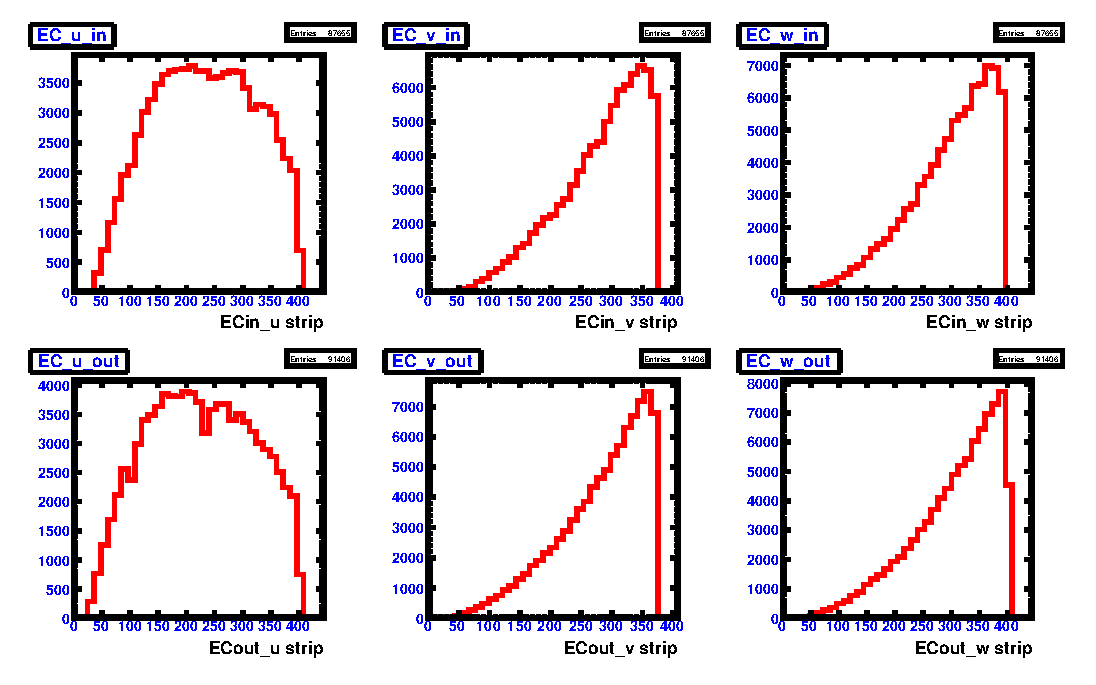
\includegraphics[width=\figwidth, height=3.5in,valign=c]{figures/calib/ec/pim_ecuvw_afterGeoFid_sec6.eps}\caption{}\label{fig:EC_IV_VI}
  \end{subfigure}%
      \caption {\abbr{EC} $u$, $v$, $w$ strips vs. $\phi$ for sector 6 with fiducial cuts and inefficient paddle knockouts applied to $e^-$ data~(\ref{fig:EC_III_VI}), notation the same as Fig.~\ref{fig:neg:ec.sec5_cut}. Number of hits vs. \abbr{EC} $u$, $v$, $w$ strips for sector 6 with fiducial cuts and inefficient paddle knockouts applied to $e^-$ data~(\ref{fig:EC_IV_VI}). Notation same as in Fig.~\ref{fig:neg.ecstrip.sec5_cut}. Image source:~\cite{clas.thesis.kunkel}}
        \label{fig:EC_cut_VI}
\end{figure}


%
%
%% % % %SECTOR 5
%\begin{figure}[!ht]
%  \centering
%  \subfloat[][]{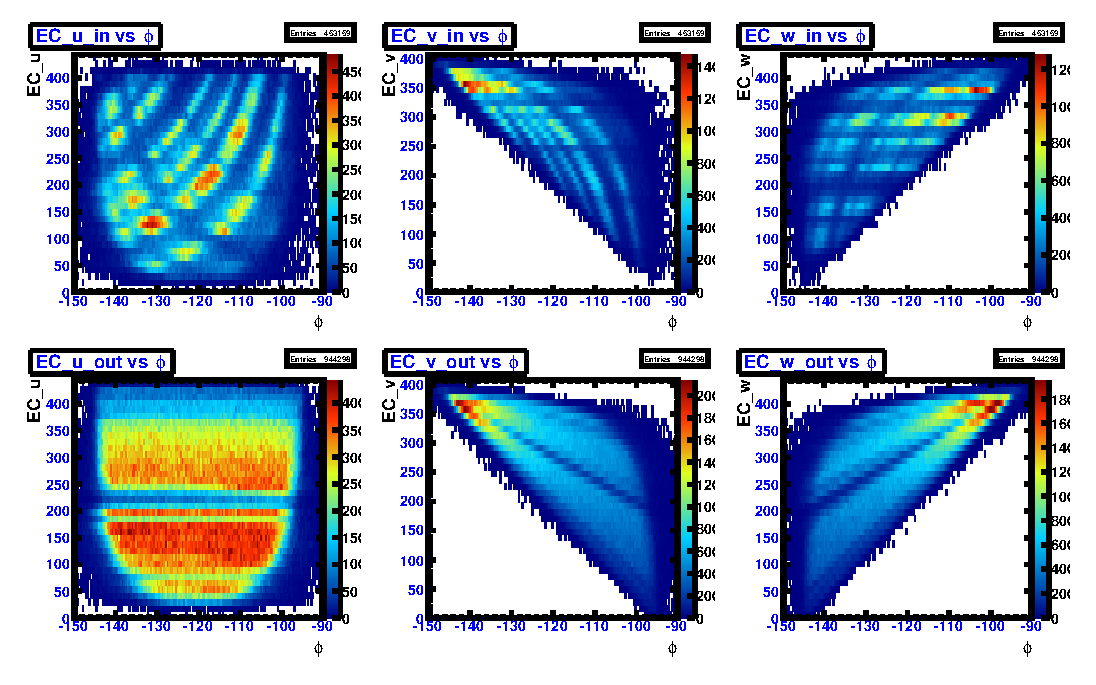
\includegraphics[width=\figwidth, height=3.5in,valign=c]{figures/calib/ec/pim_ecuvw_phi_NOKnockout_sec5.eps}\label{fig:EC_I_V}} \quad
%  \\
%  \subfloat[][]{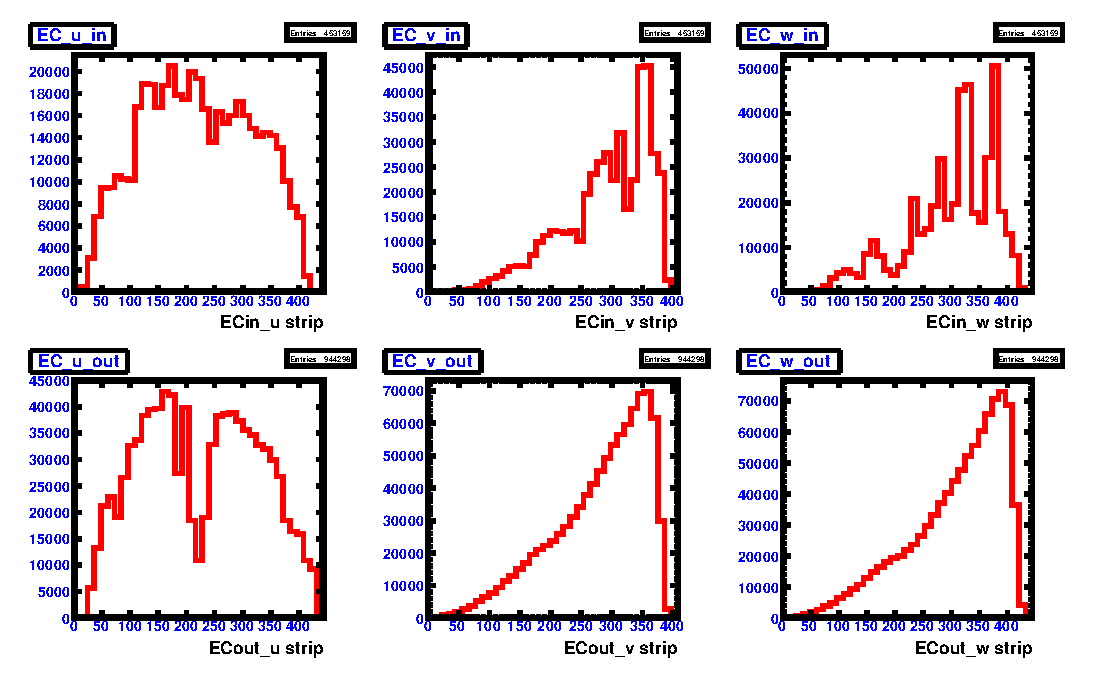
\includegraphics[width=\figwidth, height=3.5in,valign=c]{figures/calib/ec/pim_ecuvw_NOKnockout_sec5.eps}\label{fig:EC_II_V}} \\
%
%      \caption {Inefficient \abbr{EC} $u$, $v$, $w$ strips vs. $\phi$ for sector 5 in \abbr{CLAS} $e^{-} \ $ data~(\ref{fig:EC_I_V}), notation the same as Fig.~\ref{fig:neg:ec.sec5}. Number of hits vs. inefficient \abbr{EC} $u$, $v$, $w$ strips for sector 5 for $e^-$ data~(\ref{fig:EC_II_V}). Notation same as in Fig.~\ref{fig:neg.ecstrip.sec5}.}
%        \label{fig:EC_no_V}
%\end{figure}
%
%
%
%\begin{figure}[!ht]
%  \centering
%  \subfloat[][]{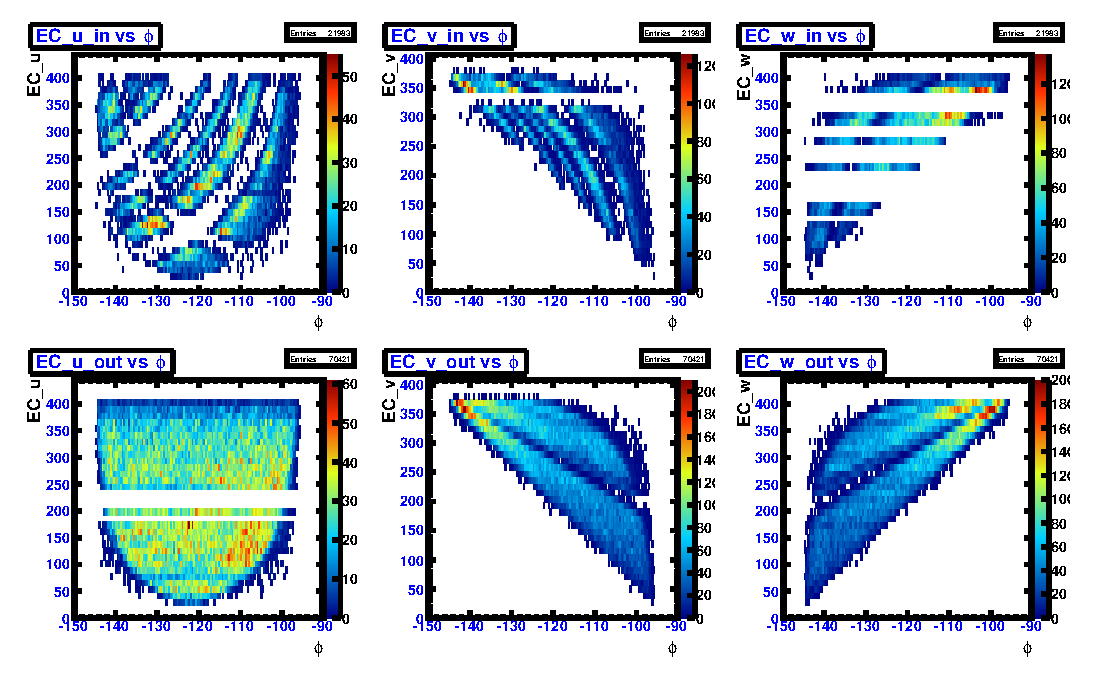
\includegraphics[width=\figwidth, height=3.5in,valign=c]{figures/calib/ec/pim_ecuvw_phi_afterGeoFid_sec5.eps}\label{fig:EC_III_V}} \quad
%  \\
%  \subfloat[][]{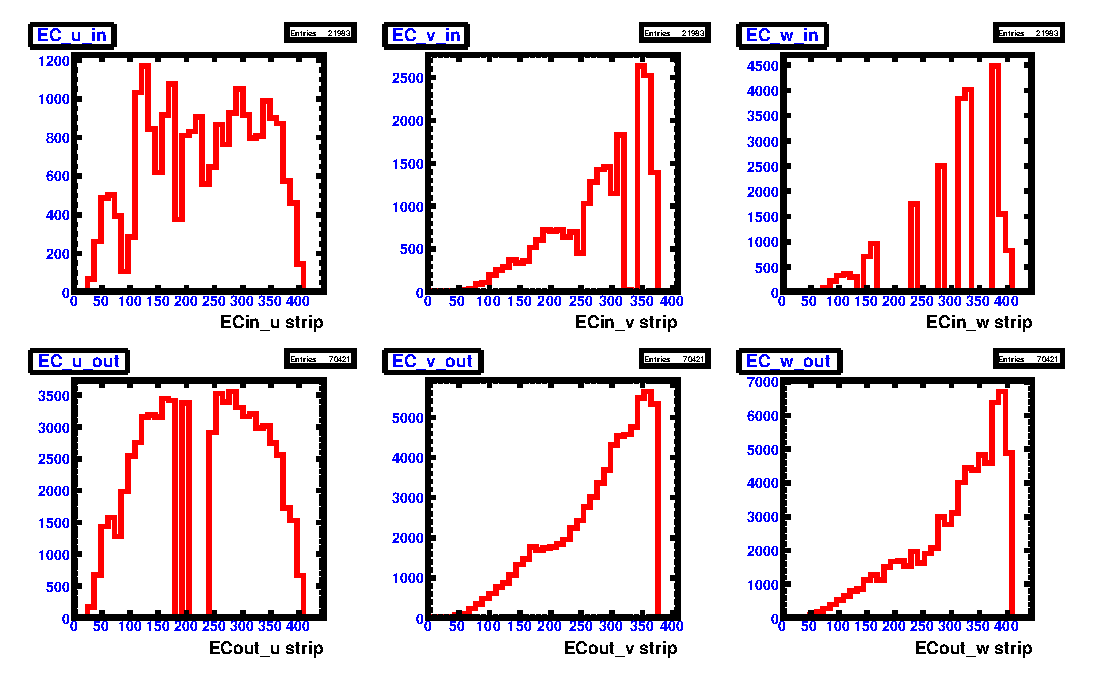
\includegraphics[width=\figwidth, height=3.5in,valign=c]{figures/calib/ec/pim_ecuvw_afterGeoFid_sec5.eps}\label{fig:EC_IV_V}} \\
%
%      \caption {\abbr{EC} $u$, $v$, $w$ strips vs. $\phi$ for sector 5 with fiducial cuts and inefficient paddle knockouts applied to $e^-$ data~(\ref{fig:EC_III_V}), notation the same as Fig.~\ref{fig:neg:ec.sec5_cut}. Number of hits vs. \abbr{EC} $u$, $v$, $w$ strips for sector 5 with fiducial cuts and inefficient paddle knockouts applied to $e^-$ data~(\ref{fig:EC_IV_V}). Notation same as in Fig.~\ref{fig:neg.ecstrip.sec5_cut}.}
%        \label{fig:EC_cut_V}
%\end{figure}
%

\FloatBarrier
The parameters for the \abbr{EC} strip cuts are listed in Tab.~\ref{tab:ec.eq} and the parameters for the good \abbr{EC} fiducial range can be found in Tab.~\ref{tab:ecfid.eq}.
\begin{table}[htpb]
\begin{minipage}{\textwidth}
\begin{center}
\begin{singlespacing}

\caption[\abbr{EC} UVW Cut Parameters]{\label{tab:ec.eq} \abbr{EC} UVW cut parameters. Table source:~\cite{clas.thesis.kunkel}}
\begin{tabular}{c|c|c}
\hline
Sector & \abbr{EC}$_{\mathrm{\emph{inner/outer}}}$  & U  \\ \hline
2 & \abbr{EC}$_{\mathrm{\emph{inner}}}$ & $96\le U\le 108  \ || \  324\le U\le 336 $   \\
3 & \abbr{EC}$_{\mathrm{\emph{inner}}}$ & $324\le U\le 336  \ || \  180\le U\le 216  \ || \  324\le U\le 337 $  \\
%
2 & \abbr{EC}$_{\mathrm{\emph{outer}}}$ & $324\le U\le 336.$ \\
3 & \abbr{EC}$_{\mathrm{\emph{outer}}}$ & $131\le U\le 142  \ || \  204\le U\le 216  \ || \  324\le U\le 336 $ \\
5 & \abbr{EC}$_{\mathrm{\emph{outer}}}$ & $180\le U\le 192  \ || \  204\le U\le 240 $  \\
%
\hline
 &  & V \\
\hline
5 & \abbr{EC}$_{\mathrm{\emph{inner}}}$  & $ 320\le V\le 342  \ || \  254\le V\le 242 $   \\
%
%
\hline
 &  & W \\
\hline
1 & \abbr{EC}$_{\mathrm{\emph{inner}}}$ & $312\le W\le 324$  \\
2 & \abbr{EC}$_{\mathrm{\emph{inner}}}$ & $396\le W\le 408$  \\
3 & \abbr{EC}$_{\mathrm{\emph{inner}}}$ & $ 396\le W\le 408$  \\
5 & \abbr{EC}$_{\mathrm{\emph{inner}}}$ & $ 336\le W\le 372  \ || \  288\le W\le 312  \ || \  240\le W\le 276$ \\
& & $  \ || \  168\le W\le 228  \ || \  132\le W\le 144$  \\
6 & \abbr{EC}$_{\mathrm{\emph{inner}}}$ & $ W\ge 396$  \\

\hline \hline%inserts single line
\end{tabular}

\end{singlespacing}
\end{center}
\end{minipage}
\end{table}
\vspace{20pt}

\begin{table}[h!]
\begin{minipage}{\textwidth}
\begin{center}
\begin{singlespacing}

\caption[\abbr{EC} UVW Good Fiducial Parameters]{\label{tab:ecfid.eq} \abbr{EC} UVW good fiducial parameters. Table source:~\cite{clas.thesis.kunkel}}
\begin{tabular}{c|c|c|c}
\hline												
\abbr{EC} Good Fiducial Range & U & V & W  \\ \hline 
& $20\le U\le 400 $  & $V\le 375.0$ & $W\le 405.0$ \\
\hline \hline%inserts single line
\end{tabular}
\end{singlespacing}
\end{center}
\end{minipage}
\end{table}
\vspace{20pt}

To perform the procedure to knock-out bad \abbr{EC} paddles, use the header file:
\begin{verbatim}
clas/users/mkunkel/clas/g12_corrections/g12_ECxyz_2uvw.hpp
\end{verbatim}
found in the SVN repository here:
\begin{verbatim}
https://jlabsvn.jlab.org/svnroot
\end{verbatim}
to convert the \abbr{EC} coordinates x, y, and z into u, v, and w \abbr{EC} coordinates. In the analysis program, the user needs to have the \abbr{EC} x, y and z coordinates, per particle, given by the \abbr{TDPL} bank for charged particles. For neutral particles the \abbr{EC} x, y and z coordinates are given by the \abbr{ECHB} bank. In the structure of \emph{clasEvent.cc} there exists functions \emph{ECpos()} and \emph{ ecPosition()} that return the \abbr{EC} x, y, and z coordinates for charged track and neutral tracks respectively. To use:
\begin{verbatim}
TVector3 partUVW = g12_ECxyz_2uvw(partECx, partECy, partECz);

double part_u = partUVW.X();
double part_v = partUVW.Y();
double part_w = partUVW.Z();
\end{verbatim}
After the \abbr{EC} u, v, and w coordinates have been calculated, use the header file:
\begin{verbatim}
clas/users/mkunkel/clas/g12_corrections/g12_EC_knockout.hpp
\end{verbatim}
found in the SVN repository here:
\begin{verbatim}
https://jlabsvn.jlab.org/svnroot
\end{verbatim}
In the analysis program, the user needs to have the \abbr{EC} inner energy deposit, \abbr{EC} outer energy deposit, u, v, w, and particle sector to perform the \abbr{EC} bad paddle knock-out. To use:
\begin{verbatim}
g12_ec_knockout(partECin, partECout, part_u, part_v, part_w, part_sec);
\end{verbatim}
which will return false if particle was knocked out, true if passed was not knocked out.

\FloatBarrier
